\section{Афинская философская школа: Сократ, Платон, Аристотель.}

Британский математик, логик и философ XX века Альфред Норт Уайтхед как-то заметил: <<Вся западная философия~---~подстрочные примечания к Платону>>. 
Продолжая его мысль, можно сказать, что вся западная наука~---~ разворачивание идей Аристотеля.

\subsection{Великое дело Сократа}

% Сократ родился в Афинах в семье скульптора Сафроникса и повитухи Фенареты. В молодости Сократ учился искусству, умел читать и писать, слушал выдающихся философов своего времени. Он занимался философией лишь устно, полагая, что запись мыслей ослабляет память. 

% Мысль Сократа дошла до нас во многом благодаря произведениям его двух самых выдающихся учеников~---~философа Платона и историка и политического деятеля Ксенофонта. Большинство произведений Платона написано в форме диалогов, неизменным участником которых как раз и является Сократ, беседующий с различными историческими и иногда вымышленными личностями. 

Сократ родился в Афинах в семье скульптора Сафроникса и повитухи Фенареты. В молодости Сократ учился искусству, умел читать и писать, слушал выдающихся философов своего времени. Сократ философствовал устно, считая, что запись ослабляет память. Его идеи сохранились благодаря ученикам~---~Платону и Ксенофонту. В диалогах Платона Сократ выступает главным собеседником.

% Сократ был выдающимся человеком своего времени, являвшим собой пример мужества на войне и рассудительности в мирной жизни. 

\subsubsection{Противостояние софистам}
% Ко второй половине V века до н.э. в Древней Греции широко распространилась практика преподавания различных полезных дисциплин. Однако в подавляющем большинстве случаев такие учителя риторики и красноречия, называя себя софистами, на самом деле никакой мудрости не учили. 

% Они брали немалые деньги за обучение мастерству спорить, умело жонглируя словам. Однако софисты не предлагали единого учения об основаниях и сами не стремились к истинному знанию. Они учили говорить не истинное по существу, но просто убеждать других в правильности своей точки зрения, лишь бы она внешне выглядела правдоподобной. 

Во второй половине V века до н. э. в Древней Греции стало популярным обучение различным полезным дисциплинам. Учителя-софисты, называя себя мудрецами, брали деньги за обучение искусству спора, но не стремились к истине. Они не предлагали единого учения, а лишь учили убеждать, делая любую точку зрения правдоподобной.

% Надёргав из различных источников умных фраз, которые могли противоречить друг другу, софисты обучали технике спора, не заботясь при этом ни о развитии совести своих слушателей, ни о том, чтобы формировать у них знания о мире, природе, государственном управлении и так далее. 

% Сократ противостоял софистам в плане как нацеленности на поиск истины, так и честности в обучении. Он никогда не брал денег со своих слушателей.
% Сократ, образно говоря, был рыцарем истины, и свою жизнь посвятил философии, как захваченности поиском истины и настоящего смысла. Ведя беседы с интересующимися гражданами, известными философами и различными софистами своего времени, Сократ сам старался выходить к истине и своим примером восстановить авторитет знания, поколебленный софистами. 

Сократ противостоял софистам, стремясь к истине и честному обучению, никогда не брал денег за свои беседы. Посвятив жизнь философии, он искал истинный смысл и пытался восстановить авторитет знания, дискредитированный софистами.

\subsubsection{Метод Сократа}

% Сократ в диалогах со своими собеседниками практикует особый метод рассуждения, получивший название майевтики, что буквально означает родовспоможение. Мыслитель говорил, что по аналогии с занятием его матери, которая помогала женщинам при физических родах, он помогает людям самостоятельно дойти до истины путём наведения их на мысль посредством вопросов, то есть помогает рождению мыслей, принимает роды души. 

% Для Сократа значимым оказываются мысли другого события, рождение мысли, причём самостоятельное. Это очень важная в педагогическом плане деталь. Настоящая философия не выдаёт какие-то готовые решения и формулы. Важно, чтобы мы сами додумались, чтобы мы сами задались вопросом и последовательно двигались в поиске ответа на него, а не принимали готовенькие мнения со стороны, которые всё равно ничего не прояснят до тех пор, пока мы сами не попытаемся осмыслить. 

% Также Сократ полагал, что настоящее может открыться только в таком откровенном диалоге, когда каждый собеседник нацелен именно на действительное понимание, а не старается кому-то что-то доказать или похвастаться своими знаниями. 

% Особенно Сократа расстраивали те, кто желают выставить себя знатоками, но на деле не разбираются в обсуждаемом. Им он спокойно и последовательно показывает, в чём и почему они ошибаются.

Сократ использовал метод майевтики~---~<<родовспоможения>> мыслей, помогая собеседникам самостоятельно прийти к истине через вопросы. Он считал, что философия не должна давать готовые ответы, а побуждать к размышлению. Истина раскрывается в искреннем диалоге, где важно понимание, а не желание доказать свою правоту. Особенно его огорчали люди, выдающие себя за знатоков, но не разбирающиеся в сути,~---~им он последовательно показывал их ошибки.

% Ну а в диалоге, кстати, слово <<диалог>> древнегреческого
% приводится буквально как через речь, через <<логос>>, искренняя беседа с друзьями
% всегда помогает увидеть истину, потому что настоящему другу мы открываемся
% полностью и доверяем. Можем признаться ему даже в том, в чём боязно себя самим,
% или благодаря его точке зрения, отличающейся от нашей, что-то новое увидеть,
% что-то важное для себя понять. Но и для полноты творчества, творчества мысли,
% нужен другой. Хотя осмыслить за каждого никто не может, как бы для легитимации
% наших идей нужен понимающий другой. Какие бы высокие идеи, какие бы чистые мысли
% мы не придумывали в одиночку, пока не обсудим их с близкими понимающими людьми,
% мы остаёмся не до конца уверены. Согласитесь? Чего-то не хватает, какого-то
% общего пространства и поддержки.

% В том числе и из-за этого Сократ не писал книг,
% считая, что живая беседа с вопросами и ответами гораздо продуктивнее, чем
% изложение какой-то концепции в тексте. 


% Примерчик, может потом оформлю его.


% А чтобы показать вам на примере работу
% сократовского метода и к тому же проиллюстрировать наши разговоры о софистах,
% выставляющихся знатоками, приведу отрывочек из первой книги Платоновского
% диалога <<Государство>>. Сократ тут беседует о понятии справедливости с
% Фросимахом, считающим себя мудрым учителем. На высказывание о том, что
% справедливость~---~это то, что пригодно сильнейшему, Сократ отвечает желанием
% разобраться. И, последовательно задавая вопроса, выясняет, что под этим
% подразумевает собеседник. Фросимах поясняет сначала, что он говорит о
% государственной власти, которая в силу своей специфики, тиранической, она
% демократической, элигархической или какая еще, устанавливает законы в
% государстве в свою пользу. Сократ спрашивает, не считаешь ли ты справедливым
% повиноваться властям? Считаю, подключает собеседник. А власти в том или ином
% государстве непогрешимы или способны ошибаться? Разумеется, способны и
% ошибаться. Следовательно, принимаясь за установление законов, они одни законы
% установят правильно, а другие неправильно. Так я, по крайней мере, думаю.
% Правильное установление властям на пользу, а неправильное во вред. Или как по-
% твоему? Да, так. Чтобы они не установили, подвластные должны это выполнять, и
% это-то и будет справедливым? Как же иначе? Иначе справедливым будет, согласно
% твоему утверждению, выполнять не только пригодное сильнейшему, но и
% противоположное, то есть непригодное. Так подумай и о том, что ты ведь признал
% справедливым выполнять также и то, что идет во вред властям и вообще тем, кто
% сильнее. Когда власти неумышленно предписывают что-нибудь самим себе во вред,
% премудрый Фросимах разве дело не обернется непременно таким образом, что
% справедливым будет выполнять как раз противоположное тому, что ты говоришь. Ведь
% здесь подчиненным предписывается выполнять то, что вредно сильнейшему. Таким вот
% разбором мнений постоянно и занимался Сократ. 

% Однако его целью совершенно не было разрушения или отрицания мнений. Часто говорят об иронии Сократа, но заключалась она ни в коем случае не в том, чтобы выставить дураком собеседника. Ирония Сократа над самим собой прежде всего. Да и в целом касается того, что удивительным образом нам откуда-то кажется буквально с пелёнок, что мы знаем, что
% такое добро, справедливость, мужество, но как только стараемся дать таким вещам
% определение, они ускользают от нас и выясняется, что мы не ведали, о чём
% говорим. Это как сейчас пропагандисты употребляют, например, слово <<свобода>> и
% призывают к ней. Однако прежде чем им доверять, ребят, задайтесь вопросом, что
% такое настоящая свобода, ведают ли они, что говорят, и можно ли извне вообще
% настоящую свободу как-то ущемить. Вот Сократа стремился благодаря такому
% внимательному всматриванию, избавляясь от ложных иллюзий, выйти к истине. В
% молодости он посетил легендарный храм в Дельфах, в котором пророчицы-жрицы, их
% назвали пифиями, предсказывали судьбу и сообщали царям и полководцам результаты
% гаданий по поводу важных событий, например, об исходе той или иной войны.
% Сократа же пифия предрекла, что он станет самым мудрым из всех известных
% эллинов. С тех пор мыслитель полностью посвятил себя философствованию и постиг
% самое надёжное знание. Думаю, вы не раз слышали в той или иной интерпретации эту
% идею. Нам дано знать достоверно лишь то, что мы толком не знаем, как всё на
% самом деле. Я знаю, что ничего не знаю, но другие не знают и этого о себе.
% Поэтому-то Сократ, не излагающий никаких концепций, по праву признавался всеми,
% как наимудрейший, ведь неразумными на его фоне кажутся все эти пафосные учителя,
% которые выдают знания о том, о чём оно достоверно невозможно, ещё и убеждает
% других в своей правоте, не разобравшись хорошенько в тех же вопросах блага,
% счастья, справедливости, свободы. 

Сократ не стремился разрушать мнения, а помогал людям осознать их иллюзорность. Его ирония была направлена не на собеседников, а прежде всего на себя. Сократ стремился благодаря внимательному всматриванию, избавляясь от ложных иллюзий, выйти к истине.

Посетив Дельфийский храм, Сократ услышал пророчество, что он~---~самый мудрый из эллинов. Это подтолкнуло его к поиску истинного знания, и он пришёл к знаменитой мысли: <<Я знаю, что ничего не знаю>>. В отличие от софистов, выдававших сомнительные знания за истину, Сократ не утверждал ничего, в чём не был уверен, и этим заслужил признание как величайший мудрец.

\subsubsection{Влияние на философию}

% Заслуга Сократа состоит не только в разработке методологического и понятийного аппарата философии, но и в переключении внимания с вопросов, касающихся только лишь рассмотрения природы и её общих законов, на проблемы человеческого бытия. Безусловно, решением этических вопросов или проблем государственного управления люди занимались испокон веков. 
% Однако Сократ, во-первых, сделал эту проблематику предметом специального теоретического рассмотрения, а во-вторых, искал ответы на вопросы о человеческой душе, добродетели, формировании знания, справедливости, власти и так далее, выводя их из единого основания. Таким образом, можно говорить, что благодаря Сократу впервые сформировалось методически проработанное философское осмысление отношения человек-мир в целом. Мыслитель придумывал как устройство мира, так и природу человека, а также разбирал специфику человеческого отношения к миру, бытийного, познавательного, этического, эстетического. 
% Наконец, благодаря Сократу философская, философствующая мысль впервые обратилась к самой себе, начала саму себя рефлексировать, то есть разбирать сам способ своего отношения к миру и свою особую методологию. 

Сократ не только разработал методологию и понятийный аппарат философии, но и переключил внимание с изучения природы на проблемы человеческого бытия. Хотя этические и государственные вопросы обсуждались и раньше, он впервые сделал их предметом теоретического анализа.

Сократ искал единые основания для понятий о душе, добродетели, знании, справедливости и власти. Благодаря ему впервые появилось методически выверенное философское осмысление взаимоотношения человека и мира. Он рассматривал не только устройство мира и природу человека, но и специфику их взаимодействия~---~познавательную, этическую, эстетическую. Кроме того, именно с Сократа философия начала рефлексировать саму себя, осмысляя собственные методы и принципы.

\subsubsection{Судьба Сократа}

% Конечно, к такой личности, как Сократ, тянулись
% молодые люди, жаждающие целостного понимания мира и своего места в нём. Однако философия такого плана предельным образом, ставящая под сомнение, даже признанные авторитетными высказываниями, из-за измеряющей мысли только с критерием подлинной истинности, не всем приходилось по вкусу. У Сократа появились завистники и политические противники тиранического склада, поскольку философ учил молодёжь самостоятельно свободно мыслить, доверяя власть сообществу рассудительных правителей, а не самодержством, стремящимся к личной выгоде и славе. Сократа ложно обвинили в том, что он развращает молодёжь и не чтит богов. В обвинение добавили и его боевой подвиг. Во время Белопонесской войны Сократ спас жизнь, вынес на себе своего молодого командира Алкивиада, которого раненого остальные бросили на поле сражения, спасаясь бегством. Впоследствии честолюбивый Алкивиад пришёл к власти и отомстил беглецам за их трусость, что, естественно, тем не понравилось. Так что Сократу обиженные и приписали в обвинение, что он якобы спас жизнь тирана. По законам Афин над Сократом состоялся публичный суд, на котором завистники обвинили его во множестве преступлений против человеческих душ. Преступления против души карались в Древней Греции самым тяжёлым наказанием даже по сравнению с убийством или кражей, за который можно было заплатить штраф, поскольку душа населилась высшим началом по сравнению с телом и физическими предметами. Несмотря на оправдательную речь, произнесенную Сократом в свою защиту на суде, философа приговорили к смертной казни. По законам Афин, приговорённый к смерти, свободный гражданин должен был сам принять яд. Его не казнил палач публично. Друзья Сократа хотели устроить для него побег, однако мыслитель со всем мужеством и достоинством принял решение суда. Ему было уже 70 лет, и хотя физически он был ещё крепок и здоров, Сократ говорил своим друзьям, что он не боится смерти и уже достаточно пожил, полностью оправдывая значение своего имени в верной власти. Мыслитель говорил, что совесть его чиста, но если такое решение о его казни вынесло свободное общество Афин, ради которого он старался всю жизнь, и за свободу и справедливость которого всю свою жизнь учил, то он обязан согласиться с приговором. 

К Сократу тянулась молодёжь, стремившаяся к пониманию мира и своего места в нём. Однако его философия, ставившая под сомнение даже признанные авторитетами истины, вызывала неприязнь у завистников и политических противников. Философ учил мыслить свободно и доверять власть рассудительным правителям, а не тиранам, что вызвало недовольство.

Сократа ложно обвинили в развращении молодёжи и неуважении к богам. В обвинение добавили и его подвиг в Пелопоннесской войне, когда он спас раненого командира Алкивиада, который позже стал правителем и отомстил трусливым воинам. Это привело к слухам, будто Сократ спас будущего тирана.

На суде философа обвинили в преступлениях против души, что считалось в Афинах тяжким грехом. Несмотря на оправдательную речь, его приговорили к смертной казни. По законам Афин он должен был сам выпить яд. Друзья предлагали ему бежать, но Сократ мужественно принял приговор. В 70 лет, будучи ещё крепким, он не боялся смерти и говорил, что его совесть чиста. Он подчинился решению свободного афинского общества, которому посвятил свою жизнь.

% Как пишет Мираб Константинович Мамардашвили, греки готовы были дать своему философу убежать. Они вообще-то не очень серьёзно собирались его убивать. Приговор был скорее ритуальным жестом,
% предполагал, что Сократ просто скроется из Афин и будет жить в изгнании. Сократ же почувствовал свою ответственность. Он считал, что малейшая неправдивость разрушает ту правду, ради которой он жил, во-первых. А во-вторых, для него важнее было быть в точке один на один со смертью, потому что только в этой точке можно знать нечто, что без этого и не в этой точке никогда не узнаешь. Что здесь имеется в виду? Сократ своим примером показал важную для настоящей философии вещь. Нельзя говорить одно, а делать другое. То есть поступок должен совпадать с тем, что ты говоришь, о чём учишь. И настоящее знание не на уровне информации находится, а на уровне, так сказать, применения в деле. Если говоришь, что справедливо~---~это так-то и так, а мужество~---~это то-то и то-то, то должен и на деле, и в жизни являть собой пример справедливости и мужества. Иначе всё, что ты говоришь об этом, никакой ценности не имеет. И жизнь, в которой говорил одно, а делать другое, окажется пустой и недостойной. Сократ говорил, что лучше уж я буду в разладе со всем миром, чем утрачу единство с самим собой. Непосредственно перед тем, как принять яд, Сократ разговаривал со своими близкими и друзьями, в том числе о том, что дело его в жизни, философия, является как бы упражнением в смерти, то есть помогает преодолеть страх смерти. Он показал это своим рассуждением. Мы боимся смерти, потому что не знаем, что происходит после неё. И, как и в любые времена, в Древней Греции существовали различные представления о загробной жизни. Так вот, Сократ говорил, что бояться нечего, если мы мужественно возьмём и разберём этот вопрос, рассуждая разумно, а не фантазируя обо всяких ужасах у себя в голове. Смерть тела означает прекращение как телесных мук, что позитивно, так и наслаждений. Но возвысив свою душу, можно и при жизни постараться отказаться от всех телесных услах, вести аскетический образ жизни, что практиковал Сократ. Что касается души, если смерть~---~это сон, то он рад, наконец, отдохнуть, заснув навечно. Если же душа бессмертна, то она может либо затем переродиться, либо попасть в божественный духовный мир вои царства мёртвых. И вот в первом случае, следовательно, душа сможет снова попасть в тело и постараться прожить не менее достойную жизнь. А во втором случае Сократ был бы рад встретиться в загробном мире и потолковать с такими людьми прошлого, как Гомер, Гесеот, Пифагор и другими выдающимися мыслителями. Сократ учил своих слушателей максимально стараться разумно рассуждать и тем самым избавлять себя как от навязываемых ложных мнений со стороны общества, так и от собственных страхов. Тогда, выходя к собственным основаниям, познавая свою душу и возвышая её, созерцая истину, можно обрести для себя надёжную опору в любом своём деле, поступке, суждении и начинании. Вот этому со времён Сократа неизменна настоящая философия и учат в педагогическом смысле, предлагая возможности для самоучения и саморазвития. Хотя, как мы на примере Сократа видим, философия~---~занятие опасное, прежде всего для самого философа. Он побуждает людей думать самостоятельно, рассуждать, переосмыслять свои представления, преодолевать стереотипы и иллюзии. И поэтому неизменно встречает сопротивление со стороны, так сказать, ленивой толпы, которая скорее отдастся в рабство готовеньким представлениям, чем будет совершать усилия, чтобы обрести действительную свободу. 

М.К. Мамардашвили отмечал, что греки не собирались всерьёз убивать Сократа~---~приговор был скорее ритуальным жестом, подразумевавшим его бегство. Однако философ отказался, считая, что даже малейшая ложь разрушает истину, ради которой он жил. Для него было важно встретить смерть с достоинством, ведь знание имеет ценность только тогда, когда воплощается в поступках. Если человек говорит об истине, справедливости и мужестве, он должен следовать этим принципам в жизни. Сократ утверждал, что лучше быть в разладе со всем миром, чем потерять единство с собой.

Перед смертью он рассуждал о философии как о подготовке к смерти, помогающей преодолеть страх. Мы боимся её, потому что не знаем, что будет дальше, но разумные размышления позволяют избавиться от беспочвенных ужасов. Если смерть~---~это просто сон, то в ней нет ничего страшного. Если же душа бессмертна, то либо она переродится, либо попадёт в мир великих мудрецов, с которыми Сократ был бы рад беседовать.

Философ учил не слепо принимать чужие мнения, а осмысленно искать истину. Познавая свою душу и возвышая её, человек обретает внутреннюю опору. Настоящая философия~---~это не передача готовых знаний, а побуждение к самостоятельному размышлению и развитию. Однако философский поиск всегда встречает сопротивление: большинство людей предпочитает удобные иллюзии истине, требующей усилий и свободы мышления.

\subsection{Философия Платона}

% Платон, выдающийся античный мыслитель, был учеником Сократа. Его имя
% означает <<широкий>>, в смысле <<широкоплечий>>. Познакомившись с Сократом в
% возрасте примерно 20 лет, Платон учился у него около 8 лет, вплоть до кончины
% Сократа. Вместе с другими учениками, после того, как учителем, Платон отправился
% в путешествие по различным образовательным центрам того времени, посетив Мегару,
% Кирену, Египет, Сицилию. А в Италии он познакомился с пифагорейцами и выкупил у
% Филолая три книги об их учении. После Платон вернулся в Афины и основал там, в
% пригороде, академию, свою философскую школу, над воротами которой, как
% утверждает предание, было написано <<Да не войдет сюда не знающий геометрии>>. Это
% означало, что Платон преподавал высшую теоретическую дисциплину и поступающие
% уже должны были обладать натренированными математическими способностями, что
% свидетельствовало об умении обобщать, выделять умозрительно форму повторяющегося
% из многообразия видимых вещей, короче говоря, о навыке абстрактно-теоретически
% мыслить. 

Платон, выдающийся античный философ, был учеником Сократа. Его имя означает <<широкий>>~---~вероятно, из-за крепкого телосложения. Познакомившись с Сократом в 20 лет, он учился у него около восьми лет, вплоть до казни учителя. После этого, вместе с другими учениками, Платон отправился в путешествие по центрам образования того времени, посетив Мегару, Кирену, Египет и Сицилию. В Италии он познакомился с пифагорейцами и приобрёл у Филолая три книги об их учении.

Вернувшись в Афины, Платон основал Академию~---~философскую школу, ставшую важнейшим центром науки и образования. По преданию, над её входом была надпись: <<Да не войдёт сюда не знающий геометрии>>. Это подчеркивало, что обучение в Академии требовало развитого абстрактного мышления, умения обобщать и выделять закономерности в многообразии явлений.

% Платон~---~первый древнегреческий мыслитель, сочинения которого дошли до
% нас полностью, сохранившись в рукописях целиком, а не в отрывках и цитатах более
% поздних мыслителей. Труды Платона представляют собой переданную в простом стиле,
% в форме диалогов, целостную философскую систему, которая охватывает как
% осмысление устройства Вселенной в диалоге тимей, так и рассмотрение проблематики
% познания в его связи с бытием, к примеру, диалоги, пармениц, минон, кратил,
% тетет, а также должного государственного устройства, государства, законы,
% политик и этических вопросов, человеческой души, любви и так далее, протогор,
% алкивят, первый, фидон, пир, федор, филек и другие сочинения. В целом, можно
% сказать, что Платон развивает через обучение у Сократа с одной стороны
% пифагорейские идеи, а с другой парменидовское внимание к бытию и его
% парадоксальности. 
% Любой платоновский диалог - это произведение
% потрясающее по своей глубине, простоте, изложении, искренности, а главное,
% актуальности для нас сегодняшних. 

Платон~---~первый древнегреческий философ, чьи сочинения дошли до нас в полном виде, а не в отрывках или цитатах других мыслителей. Его труды, написанные в простом стиле и представленные в форме диалогов, образуют целостную философскую систему. В них рассматриваются вопросы устройства Вселенной (например, в диалоге Тимей), проблемы познания и бытия (Парменид, Менон, Кратил, Теэтет), вопросы государственного устройства (Государство, Законы, Политик) и этики (Протагор, Алкивиад, Федон, Пир и др.).

В своих работах Платон сочетает идеи пифагорейцев с парменидовским вниманием к бытию и его парадоксальности. Каждый диалог Платона~---~произведение, отличающееся глубиной, ясностью изложения, искренностью и остающееся актуальным и для современного читателя.

\subsubsection{Онтология Платона}

% Учение об идеях или разделение на мир идей и мир
% вещей. Эйдос, который обычно переводят как идея или синонимами образ, вид, форма,
% действительно является одной из основных категорий философии Платона. Идея вещи
% не содержится в видимом мире как какая-то отдельная специфическая сущность, но
% как бы представляет собой невидимую, обычному зрению матрицу, как бы исходный
% код, который задает форму, оформляет, определяет чувственно воспринимаемые вещи.
% Например, в мире мы встречаем совершенно разнообразных лошадей по пародии,
% красу, характеру и так далее. Но, тем не менее, мы в уме оперируем идеей лошади
% как обобщающим понятием, которое, с одной стороны, не совпадает ни с какой-то
% конкретной лошадью, ни с их совокупностью, а с другой без них в мире не
% встречается. Но может быть абстрактно помысленно в нашем уме. Давайте сразу
% оговоримся о переводах слова эйдос. Вид в случае с конями неплохой перевод
% эйдоса, потому что, во-первых, A-D-N-I, это тоже в русском однокоренное видеть,
% с оттенком распознавать, постигать. И, во-вторых, сразу понятно, есть вот эти
% конкретные лошади, а есть биологический вид или род лошадей. Образ и формы
% совсем плохие переводы, ведь лошадь вообще никак не нарисовать, зримо не
% представить. Будут только форма или образ какой-то определенной лошади. Даже
% условной линией нарисована это не вид лошадей, а конкретная картинка. То есть
% эйдос лошади~---~это скорее абстрактный образец для всех возможных, в том числе
% нарисованных, слепленных или иначе созданных лошадей, чем визуальный образ их
% обобщающий. Ну или, чтобы понятнее было, медные предметы или кусок меди, мы
% можем представить, они будут иметь какую-то форму, по-гречески форма морфе. А
% вот медь вообще, медь как таковая, зрительного образа не имеет. Понятно, да? Мы
% можем только обозначить эйдос, химический элемент медь. Но вы знаете прекрасно
% со школы, что это чистая абстракция, вид атомов с зарядом ядра, каким-то 29, и
% средней атомной массой 63,5. Но и слово
% идея в современном нашем языке уже тоже не очень хороший перевод эйдоса,
% потому что у нее есть второе значение, гораздо чаще нами используемое, когда мы
% говорим, у меня возникла идея. Или, например, это идея Канта, в смысле положения
% его философии. Однако и словом вид, переводить эйдос не во всех случаях
% получится, потому что помимо рядов предметов и явлений, которые мы реально в
% мире встречаем, в каких-то уникальных воплощениях, есть и красота, и добро, и
% мужество, и справедливость, и зло, и безобразные, и трусость, и несправедливые, много еще подобных категорий, которых самих по себе, мы уже не раз об этом говорили, в мире не встретить. При этом нам доступно оценивать человека как мужественного или недоброго, или злого, и так далее. И вот сами по себе подобные понятия, которые тоже могут быть общими для многих реальных людей, или, например, лошадей, это тоже эйдосы. Единое и многое части, целое, четное и нечетное, качество, количество, материя, это все тоже эйдосы. Так что давайте их так и называть, этим греческим словом, или, как наиболее принято, платоновскими идеями. Собственно, где они, если в мире самих по себе эйдосов нет? Платон логичен, значит, они вне мира. Поскольку они чисты и предельно абстрактны, скорее всего, они в божественном мире, в мире возвышенного, и оттуда они как бы проецируются на материю, придавая вещам нашего мира определенные характеристики.

Учение Платона об идеях или разделение на мир идей и мир вещей основывается на концепции эйдоса (эйдос), который обычно переводят как <<идея>> или синонимами <<образ>>, <<вид>>, <<форма>>. Эйдос является одной из центральных категорий философии Платона. Важно понимать, что идея вещи не является отдельной сущностью, присутствующей в видимом мире. Вместо этого, она представляет собой нечто невидимое, как бы исходный код или матрицу, которая формирует и определяет чувственно воспринимаемые вещи.

Например, в нашем мире мы встречаем много различных лошадей с разными породами, цветами, характерами и так далее. Но в нашем уме существует идея лошади как обобщённое понятие, которое, с одной стороны, не совпадает с какой-то конкретной лошадью, и с другой~---~невозможно встретить без этого понятия. Идея лошади существует как абстракция в нашем уме.

% Когда мы переводим слово "эйдос", слово "вид" подходит в случае с конями, так как оно подразумевает возможность различать и постигать. Однако "образ" или "форма"~---~это плохие переводы, потому что лошадь невозможно нарисовать или представить в полном виде. Эйдос лошади скорее будет абстрактным образцом для всех возможных лошадей, а не конкретным визуальным изображением.

% Точно так же, как медь не имеет зрительного образа, эйдос меди~---~это скорее химический элемент с определённой структурой, а не визуальный образ. Также слово "идея" в современном языке имеет другое значение, например, когда мы говорим о какой-то концепции или мысли, что делает его неточным переводом эйдоса.

Помимо конкретных предметов, существует и множество категорий, таких как красота, добро, мужество, справедливость, которые не имеют материального воплощения, но мы можем оценивать их через реальные вещи или действия. Все эти категории тоже являются эйдосами, или платоновскими идеями.

Платон логично выводит, что такие идеальные эйдосы не находятся в мире вещей. Поскольку они чисты и абстрактны, они, скорее всего, существуют в божественном мире и проецируются на материю, придавая реальным вещам их характеристики.

% Однако Платон прекрасно понимает всю проблематичность
% такой концепции и сам в своих диалогах, особенно в Пармениде. ее критикуют, или,
% вернее сказать, рассматривают парадоксы и затруднения, которые возникают, если
% мы примем, что так оно и есть, что эйдосы, пребывая где-то отдельно, являются
% матрицей для реальных вещей нашего мира. В диалоге Парменид молодой Сократ
% встречается с главой и другими представителями элейской школы. Вспоминайте наш
% предыдущий вопрос с прошлой лекции. Зинон читает афинянам свои сочинения, и
% далее Сократ с ним и уже на тот момент старцем Парменидом вскрывают опори
% относительно мира идей. Могут ли существовать эйдосы отдельно от того ряда
% конкретных вещей, которые им подобны, пытает Парменид юного Сократа. Если каждый
% эйдос существует отдельно, един и целостен, то как он может разделяться многими
% вещами? Если он покрывает эти вещи, как плащ, его можно накрыть несколько
% человек, то каждая вещь будет находиться только под какой-то частью эйдоса, как
% каждый человек накрыт только частью плаща. Но если у эйдоса есть части, то он
% состоит из множества, значит, он в себе не един, значит, и каким-то вещам может
% достаться больше кусочков эйдоса, а каким-то меньше? Разве может неоделимая,
% абсолютно чистая, абстрактная идея быть многим, разделяться на части, не быть
% единым, а следовательно, самой собой? Каким образом вещи причастны идеям? Мы
% тоже толком не можем сказать, раскрыть этот механизм. Да и что же, если какой-то
% человек лицом похож на лошадь, что же он от части причастен и эйдосу лошади?
% Человек и конь, вроде бы, вид взаимоисключающий. Кроме того, откуда мы об
% эйдосах имеем представление, если они вне мира? Кто нам сказал? Не получается ли
% так, что мы просто видим в мире ряд похожих вещей и придумываем сами для них
% названия? Да и если эйдосы так божественны и возвышенны, могут ли они быть у
% всего в нашем мире или только у хороших, возвышенных вещей? А у мусора,
% например, или в грязи тоже есть соответствующие эйдосы? Когда парменит вот об
% этом обо всем спрашивает, Сократ признается, что и сам теряется под этого
% механизма. Когда думает об этом, признается, что по-честному не знает, видит все
% эти противоречия, но не знает, как их разрешить. 

% Вот. Вы теперь видите, какой
% настоящий Платон, что он в своих текстах излагает? Поэтому, ребят, не впадайте в
% так называемый вульгарный Платонизм, согласно которому наш мир как бы ущербный,
% несовершенно слепок с того идеального мира эйдосов и дей. Нет ведь идеально
% мужественного человека, нет ведь абсолютно красивой и добротной во всем лошади.
% Это не абстрактные вещи, а то, что в каждом из нас сидит. Присмотритесь к себе,
% как мы хотим от окружающих, чтобы они были согласны нашим представлениям
% идеальными. Как от себя мы хотим быть с идеальным телом, быть постоянно
% радостными и продуктивными. Это очень опасно. Почему? Мы себя этим истязаем,
% копим зависть, обиды, которые нас разрушают. Надеюсь на этот образцовый мир, как
% будто чистые эйдосы могут прийти и быть вместо вещей в реальном мире. Но нет,
% ребят, мы все и все в мире несовершенно. И это нормально. Это тоже надо увидеть,
% принять и полюбить, в том числе себя, такими, какие мы есть. Безусловно, мы не
% только можем, но и должны стремиться к красоте, здоровью, мужеству, мудрости.
% Однако важно при этом видеть всю полноту нашей реальности и понимать, что самих
% по себе чистых идей в действительности не достичь. Не надо от себя хотеть
% совпасть с идеалом. Это гонка Ахиллеса за черепахой. Если не принимаете
% парадокс, он вас возьмет в оборот и зарасходует. Стоит взглянуть на наш мир с
% пренебрежением и мы подрубаем единственный сук, на котором можно сидеть. Он
% единственное, что у нас есть. Ведь мира, который там, у нас нет. Тот мир в нашем
% воображении. Он на самом деле несравненно нищее, чем самая жалкая вещь этого
% мира. Как самая красивая фотография роскошно сервированного стола, хуже, чем
% самая маленькая завялая морковка. Понимаете, да? Не исключено, что есть какие-то
% другие божественные, чистые, абстрактные миры. Возможно. Мы не знаем. Но
% настоящий мир для нас только вот этот. Можно иметь в уме идею 100 рублей, но не
% имея их в действительности ничего не купишь. И вот настоящий Платон такое
% понимал и в своих трудах парадоксы разбирал, а не конструировал красивые мифы,
% которые из его философии понаделали потом те, кто его не понял. Настоящий Платон
% это один сплошной вопрос. А неготовенькая, непротиворечивая концепция. Сплошные
% парадоксы на каждом шагу. Мы можем неуклюжие ответы находить под наше хромающее
% суждение, подсовывать подпорки, рискуя, как Сократ Пармениду говорит, потонуть в
% бездонной пучине пустословия. Чего бы, естественно, ищущим истину не хотелось.
% Но как бы мы не упорствовали, опори непроходимы. Вокруг настоящих самых главных
% вещей они неизбежно будут возникать. И тут самое главное~---~выбрать только одно
% из пары противоположностей. Мужественно уметь, как Сократ, по-честному признать.
% Да. О таких вещах у нас нет и не может быть непротиворечивой теории. Нет и не
% может быть знаний, но чудесным образом нам дано их видеть, иметь с ними дело и
% распознавать в мире ту же красоту, доброту, справедливость. Это то, что потом в
% 15 веке Николай Кузанский назовёт <<знающее незнание>>. 

% И вот вся настоящая
% античная философия~---~это школа незнаний. Не в смысле необразованности, а
% напротив, это максимально возможное знание. Сами школы не случайно так
% назывались. От греческого <<схоле>>~---~остановка, ну не автобусная остановка, а
% пауза, отстояние, зависание над вопросом проблемы. Это состояние о механии,
% когда приходится остановиться, отложить повседневные все бытовые дела,
% остановиться и подумать. И в средние века с холастикой от этого же слова будет
% называться такое мышление, которое старается логичным образом разобрать подобные
% глубокие вещи. И несколько столетий подряд самые выдающиеся средневековые
% исследователи будут биться над проблемой универсалий, тех самых общих понятий,
% родов и видов. Реально они существуют как матрица для вещей видимого мира, или
% это просто имена, название, которое мы сами в виде похожей предметы придумали
% для их обозначения в языке. После того, как мы хотя бы краешком глаза заглянули
% в самый трудный платоновский диалог про Минит, становится ясно, что Эйвисы не
% то, что подошло бы на роль самого фундаментального антологического основания в
% философии Платона. Более того, нельзя сказать, что это единая с большой буквы,
% которая мы вроде бы поместили с вами в антологические основания всей эпохи на
% прошлой лекции. Если единое мы каким-то образом постигаем через многое,
% например, видим умом лошадность всех лошадей, то значит, оно существует во
% многих и уже не будет единым, значит, оно существует через другое и уже не само,
% а вот что само. Это главный, наверное, вопрос всей афинско-философской школы.
% Вопрос о таком предельном основании, которое и единое, и многое делает самими
% собой и всё остальное. Эйдосы таковыми и вещи в мире, каждую уникальны. Об этом
% платоновский диалог Алкивиад I, хотя начинается всё с далёких, казалось бы, от
% фундаментальной антологии вещей. Сократ идёт в дом к любимому ученику и
% встречает его на пороге того самого, которого он потом спасёт на поле боя,
% красавца Алкивиада. Ему только исполнилось 20 лет, и он спешит в народное
% собрание. С этого возраста юноша считался совершеннолетним в Древней Греции и
% как свободный гражданин мог участвовать в обсуждениях дел полиса. Собирается
% идти убеждать сограждан по вопросам войны и мира, определять политику своего
% города-государства. И Сократ заговаривает с Алкивиадом, мол, откуда тот знает о
% таких вещах, как, например, благо для граждан и справедливость государственной
% политики. У кого? Когда научился? В ходе беседы выясняется, что Алкивиад думал,
% что знал с детства, с рождения, но что такое благо и справедливость, растерялся
% сейчас Сократу ответить. Сократ показывает ему, что нельзя доверять такие важные
% дела тем, кто не знает, не понимает в них, как нельзя доверить, скажем,
% управление кораблем тому, кто прежде не обучился этому. С государством так же.
% Что же нужно познать, чтобы управлять людьми ради общего блага? Гной за Сеофтон,
% узнай себя. Сократ говорит, легко ли познать самого себя, ведь не первый же
% встречный начертал это на Пефийском храме. Алкивиад понимает, что дело это
% трудное, для этого нужно знать природу человеческой души, понимать, что есть мы
% сами, что делает каждого самим собой. 

Вся настоящая античная философия~---~это \textbf{школа незнания}, но не в смысле необразованности. Это знание, которое осознаёт свои пределы и стремится к максимально возможному пониманию. Философия, особенно в Древней Греции, была сосредоточена на поиске истины, что невозможно без глубокого размышления, паузы в повседневной жизни. Именно от греческого слова <<схоле>>~---~остановка, пауза~---~происходит термин <<школа>>, который отражает необходимость приостановить повседневные дела и сосредоточиться на важных вопросах.

% Индивидуально, свое собственное~---~и есть предельное
% всеобщее основание. У Платона оно называется самое само, в оригинале авто то-авто. То, что течет через все и делает каждое сущее самим собой. 
% Оно первичнее и единого, потому
% что делает его ничем иным, как единым. Бытие и небытие тоже вторичны, поскольку они, соответственно, не что иное, как бытие и небытие. Чтобы быть самими собой, нужно такое первоначальное, самое само. Так что у Платона, а не у Парменида, впервые названы максимально предельные основания, самое свое собственное. 

\textbf{Свое собственное}~---~это предельное основание, у Платона называемое <<самое само>> (авто-то-авто), то, что проходит через все и делает каждое сущее самим собой. Оно первичнее единого, так как делает его ничем иным, как единым. Бытие и небытие вторичны, поскольку они не что иное, как бытие и небытие.

% Но мы уже в третьей теме заглянули, в парадоксы своего собственного, тут не будем их повторять. Самое главное для нас сейчас в разговоре о философии Платона
% пометить. Это наиболее фундаментальное антологическое основание, которое, ребят,
% с тех времен не поменялось. И вся самая современная философия XXI века все о том
% же. Дальше Парменида и Платона не шагнуло, ищет свое и не находит, лишь
% констатируя его ускользание от концептуализации. Однако, каков бы ни был
% антологический статус Эйдосов, 


% Платон приходит к тому, что мы познаем благодаря
% умению выделять идею вещи, то есть в уме созерцать ее Эйдос и оперировать им. Платон задается вопросом, откуда же берутся у нас в голове эти идеи, когда
% очевидно, что в мире мы их непосредственно не видим. Откуда научаемся мы им?
% Ладно еще, когда дело касается обобщающего понятия для видимых предметов, будь
% то гора, лира, собака или лошадь. Откуда мы имеем представление о таких
% совершенно незримых вещах, как красота, добро, справедливость, мужество, единое
% бытие, качество, количество, душа, свобода и так далее. Мы можем иметь дело со
% справедливым решением, справедливым государственным строем, справедливым
% человеком, однако не можем в мире увидеть справедливость саму по себе как
% таковую. 

Платон приходит к выводу, что мы познаем, выделяя идею вещи, \textbf{созерцая её эйдос} в уме и оперируя им. Он задается вопросом, откуда у нас возникают эти идеи, если мы их не видим в мире. Это касается не только обобщающих понятий для видимых предметов, но и таких абстрактных вещей, как красота, добро, справедливость, мужество, душа и другие, которые нельзя увидеть как самостоятельные сущности в мире.

\subsubsection{Гносеология и антропология Платона}

% Это уже само по себе парадоксальные свойства нашего познания, поэтому
% обсуждать подобные проблемы вслед за Сократом Платон берется методом
% диалектического исследования, то есть движение мысли в пространстве между
% противоположностями. Следуя происхождению слова диалектика, легко заметить, что в основании метода работа с взаимодействием, взаимно обратимым движением через двойную диалектику лектике. Поэтому диалектика работает с противоположными лексическими парами категорий, вскрывая их взаимную связь. Однако надо помнить, что не все можно расписать на противоположности. Истинными противоположностями можно назвать только что-либо и его отсутствие. Например, о противостоянии материи и формы говорить не совсем корректно. Это разные категории, но отнюдь не противостоящие друг другу. Форма противостоит не материи, а отсутствию формы бесформенному. 

Платон, как и Сократ, рассматривает парадоксальные свойства нашего познания с помощью диалектики~---~метода, основанного на движении мысли через противоположности. Диалектика работает с парами категорий, выявляя их взаимную связь. Однако важно помнить, что не все можно свести к противоположностям. Например, материя и форма не противостоят друг другу, а форма противостоит отсутствию формы.

% Аристотель в своей физике приводит по этому поводу пример. Образованность и невежество противоположности, представляющие собой форму образованность и решенность этой формы необразованности или невежества. Человек же, которому может быть присуще качество образованности или у которого это качество может отсутствовать, не имеет противолежащего, но в данном случае играет роль подлежащего, лежащего в основании. Так вот, изменяться друг в друга сами по себе противоположности не могут. Они как категории как бы зафиксированы и независимы друг от друга. Однако человек, как подлежащее изменению, субъект, может из невежды стать образованным. Это пример вам для понимания, что такое античный диалектический метод.

% сводить любое
% различие к противостоянию и противоположности~---~не совсем верно. Это сужает
% наше видение реальной ситуации, в которой всё гораздо тоньше. Так вот, благодаря
% этому методу Платон приходит к тому, что такое наше знание и понимание смысла
% идей, эйдосов, видимых вещей и высших категорий происходит из самой души,
% которая до попадания в человеческое тело созерцала эти чистые идеи в
% божественном мире. То, что мы узнаём в мире, тогда является результатом
% припоминания нашей душой тех эйдосов, которые она уже созерцала. Платон
% доказывает это потрясающим образом на примере обучения геометрии. Человек и так
% уже как бы в свёрнутом или спящем виде имеет всё возможное знание и
% представление. И совершенно не знающие, например, геометрической теоремы докажут
% её и выведут необходимые следствия, если перед ним просто поставить определённым
% образом задачу. В этом можно усмотреть и переосмысление роли учителя любого в
% любом деле, а не только в философии. Для нас и так уже всё есть. Всё, что только
% возможно, знать и понимать для нас открыто. Задача учителя заключается тогда
% вовсе не в том, чтобы выдать какую-то информацию или воспроизводить известное
% знание, а в том, чтобы так суметь настроить ум слушателей, чтобы они сами
% задались вопросами и сами развернули собственный путь к добыче знания, к истине.
% Она и так всегда уже есть в нашей ситуации, просто из-за множества мнений,
% социальных стереотипов, иллюзий мы можем её не видеть, не замечать или без
% должного логического разбора принимаем мнимое, расхожее за истину. Задача
% философии расчистить наше видение от этих мешающих конструкций и помочь узреть
% истинно. 

Платон, используя диалектический метод, утверждает, что наше знание и понимание идей происходят из самой души, которая до воплощения в теле созерцала чистые идеи в божественном мире. Знание, которое мы получаем в жизни,~---~это \textbf{припоминание} этих идей. Например, на уроках геометрии ученик, не зная теоремы, сможет доказать её, если ему правильно поставить задачу.

% Данная концепция подразумевает и другие гносеологические следствия,
% вернее, даёт представление о других гносеологических основаниях античного
% видения. Эйдосы, как незримые, но постигаемые умом образы вещей, это аналог
% пифагорейского числа, которые не усматривали вещи, как некий первичный код-
% форму, благодаря которому вещь перед нами предстаёт именно такой, именно такого
% вида. Платоновские идеи мыслились именно как такого рода оформляющее начало, без
% которого в мире не было бы упорядоченности и завершённости предметов. Так, в
% античном миропонимании укореняется эйдетическое понимание причинности, то есть,
% когда мы в рамках античного типа мышления рефлексируем, задуваясь вопросами о
% причинах данного положения вещей. Мы приходим как раз к идее Эйдосу как
% определяющему принципу. Например, если мы зададимся вопросом, почему человек
% заболел, сегодняшние мы будем выстраивать линейно-комплексные причины и связи,
% отвечая, потому что его продуло, иммунитет ослаблен, в организме
% распространяются болезнетворные микробы. Вывод, здесь и сейчас надо бороться с
% микробами. Древний грек ответил бы иначе на вопрос, почему человек заболел. В
% данный момент этот человек соответствует идее болезни. Безусловно, греки
% понимали временность любого положения дел, всё течёт, всё изменяется, поэтому
% для выздоровления нужно было стремиться к противоположной идее, диалектически к
% эдосу здоровья. Как лечиться в таком случае? Подождать. Тело выздоровеет само,
% потому что по природе стремится к здоровью, но ему можно помочь,
% поспособствовать к выздоровлению. Сон, покой, соответствующее питание и питьё,
% умеренность во всём. А ещё обязательно заранее, чтобы не попасть в лапы эдосу
% болезни, нужно для своего тела практиковать стремление к идее здоровья,
% закаляться, упражняться, хорошо и сбалансированно питаться, а уж когда заболел,
% то и не нагружаться и не требовать от своего тела обычной работоспособности,
% поскольку силы тратятся на восстановление организма. Интересно, что в рамках
% такого целостного подхода и такой рациональной системы воспитания, здоровье у
% древних греков было отменным. Сейчас мы все эти вещи другим путём объясняем и
% лечим часто не человека, а проявление болезни, симптомы, поскольку исходим из
% других антологических принципов. Для теоретически настроенного ума никакой
% проблемы не предоставляет проследить все причины следственной цепочки.
% Естественно, и древние греки это могли, но они всматривались в первые причины и
% самые фундаментальные основания так надёжнее. Поэтому эйдетическая причинность
% не хуже, она всё равно во всём есть, независимо от того, на чём нам сегодня
% привычнее концентрировать внимание и как привычнее рассуждать.

Концепция Платона предполагает, что эйдосы~---~это незримые, но постигаемые умом образы вещей, аналогичные пифагорейским числам, которые определяют формы вещей. Эти идеи~---~оформляющее начало, без которого мир был бы неупорядоченным. В античном мире \textbf{причинность} понималась через эйдосы, и вопрос о причинах чего-либо выводил к идее определяющего принципа. 

Например, при болезни древние греки рассматривали её как соответствие идее болезни, а выздоровление~---~как стремление к идее здоровья. Лечение включало покой, правильное питание и физические упражнения. В отличие от современного подхода, ориентированного на симптомы, древний подход фокусировался на первых и фундаментальных причинах.

% Какова природа человека?
% Что такое человек в своём существе? Ясно, что мы очень похожи на животных, тоже
% являемся живыми существами с телом и душой. Когда нас с одной стороны внешне
% отличают телесные особенности, а с другой способности души. Животные ведь все
% способны ощущать, воспринимать, чувствовать, испытывать какие-то эмоции, страхи,
% но человеческая душа имеет также и высшую способность к осмыслению своих чувств
% и переживаний, которые обычно называют разум. Уподобляя душу человека парной
% упряжки с возничьем во голове, Платон метафорически описывает структуру
% человеческой души как состоящую из трёх составляющих. Чувственно воспринимающее
% как бы самое низменное начало это в его образной аналогии плохой конь, который
% не слушается, стремится к чувственным страстям, удовольствиям и усладам тела.
% Яростно волевое начало это хороший конь, который слушается возничьего и
% представляет собой благородное волевое начало души. Иррационально-рассудительное
% это возничий разум, который должен мудро управлять своей колесницей, сдерживая
% плохого коня и воспитывая в нём покорность, скромность, смиренность, а также
% направляя в нужную сторону хорошего коня. 

Природа человека включает в себя тело и \textbf{душу}, и хотя мы похожи на животных, наша душа обладает высшей способностью~---~разумом, который осмысляет наши чувства. Платон метафорически описывает структуру
человеческой души: чувственное начало (плохой конь), волевое начало (хороший конь) и разум (возничий), который управляет этими началами, сдерживая плохого коня и направляя хорошего.

\subsubsection{Этика и политическая теория Платона}

% Идеалы строгости и разумности,
% справедливости и мудрости с точки зрения Платона также должны руководить жизнью
% государства. В одном из своих самых объёмных диалогов под названием
% <<Государство>> Платон задаётся множеством вопросов, касающихся существа
% государства, его возникновения, должной организации, власти, справедливости,
% воспитания и так далее. Одной из основных идей данного произведения является
% поиск единого принципа, в соответствии с которым могло бы быть построено сильное
% государство со справедливой системой управления, которое заботилось бы о благе
% всех своих граждан, а не какой-то из частей общества. Платон находит такой
% единый принцип. 

В диалоге <<Государство>> Платон исследует природу государства, его организацию, власть и справедливость. Основная идея произведения~---~поиск единого принципа, который мог бы создать сильное государство с справедливой системой управления, заботящуюся о благе всех граждан, а не только отдельных групп.

% Единственный закон, который непрестанно по сути должен
% выполняться для поддержания счастливого единого государства, это чтобы каждый в
% государстве следовал своему призванию. В этом произведении Платон высказывает
% мысль о том, что все люди по своим способностям от природы различны, поэтому,
% чтобы человек был счастлив, он должен развивать свои способности, исполняться в
% том, к чему у него от природы лежит душа. Короче, исполняться в своем
% собственном, в полном согласии с онтологическим основанием, которое самое-само,
% Платон устами Сократа, помните, выше я вам стирала кусочек из его разговора с
% Форсимахом, дает прекрасное определение справедливости, заниматься своим делом и
% не вмешиваться в чужие. Так же, как пищу, должен готовить человек, у которого
% способности к вкусу и сочетанию, умелому обращению с продуктами, гончарные
% изделия должен создавать человек, которому интересно работать с глиной и он ее
% чувствует. Одежду должен делать человек, интересующийся тканями,
% соответствующими способами пошива и обработки, материалами и так далее. Так и
% стражем, воином должен быть не любой человек, а лишь тот, кто по призванию всем
% сердцем любит справедливую борьбу и состязание. И уж тем более управлять
% государством должен управленец по призванию, мудрый, рассудительный, а не
% тщеславный человек, старающийся обладать властью, но другими ради собственной
% выгоды. Если люди, стоящие на страже законов и государства, таковы не по
% существу, а только такими кажутся, ты увидишь, что они разрушат до основания все
% государство и только у них от них будет случай хорошо устроиться и процветать.
% До того, пока мы не прислушаемся к этому и сами не постараемся всеми силами
% соответствовать своему собственному, развивая данные природоспособности, боюсь,
% из года в год продолжить сбываться это пророчество Платона. Тогда что же делать?
% Каждого из граждан надо ставить на то одно дело, которому у него есть
% способности, чтобы, занимаясь лишь тем делом, которое ему присуще, каждый
% представлял бы собой единство, а не множество, так и все государство в целом
% станет единым, а не множественным, пишет Платон. в этом его сочинение просто
% кладезь полезных и продуктивных идей по поводу войны и мира, врагов и друзей,
% нашего способа мыслить и познавать, о том, что женщины тоже должны исполняться
% согласно своему призванию, как и мужчины, учиться работать наравне с ними, даже
% если женщина по призванию воин или политик. В IV век до нашей эры, а до западной
% цивилизации только через 25 столетий после Платона дошло, что женщина тоже
% человек. Там такой коммунизм с общностью жены детей, что Марксу даже и не
% снился. Почитайте сами, я, к сожалению, не успеваю вам все эти интересности
% рассказать. 

Платон утверждает, что для счастья каждого гражданина важно заниматься тем, к чему он предрасположен от природы, развивая свои способности. Для справедливого общества каждый должен исполнять свою роль: ремесленники, воины, управленцы~---~все по призванию. Платон также подчеркивает, что для стабильности государства важно, чтобы люди занимались лишь тем, в чем они способны и к чему имеют природные склонности. Он утверждает, что женщины должны иметь такие же права и возможности, как мужчины, включая участие в военном или политическом деле.

% Мыслитель также приходит к отождествлению бытия и блага, как и высшего принципа всего мироустройства. Платон полагает мир сотворенным в свете идеального от слова идеи божественного замысла и устроено, задумано все наилучшим образом. Все есть так, как должно быть все благо. Благо понималось как единый основополагающий принцип. Платон соотносил эту, казалось бы, этическую категорию и с познанием, то есть с областью гносеологии. Как мы с вами уже разобрали и прочувствовали, на прошлом занятии в античной философии все связано. Ведь в нашей жизни вопросы о человеческой душе порождают вопросы о разуме и познании, которые в свою очередь отсылают к бытийному устройству всего сущего. Так и философия Платона представляет собой единую целостную систему осмысления отношений человек-мир. 

Платон отождествляет бытие и благо, считая их высшим принципом мироустройства. Он утверждает, что мир сотворен в свете идеального божественного замысла и устроен наилучшим образом. Благо для него~---~это основной принцип, который связывает этику и гносеологию. В философии Платона всё взаимосвязано: вопросы о душе, разуме и познании ведут к размышлениям о бытии, и вся его философия представляет собой единую систему осмысления отношений человека и мира.

% И вот сведение этической и онто-гносеологической проблематики в единое целое получило название этического рационализма. Вспоминайте, в основаниях эпохи античности мы с вами это тоже уже отмечали на предыдущей лекции. Теперь чуть подробнее раскроем эту позицию, в соответствии с которой поступки совершаются человеком, исходя из рациональных оснований. Сами по себе категории и их пары противоположностей, такие как добро и зло, справедливое и несправедливое, прекрасное и безобразное и подобное представляют собой как бы пустые формы. Они зависят от наполнения в конкретной реальной ситуации. Нельзя сравнивать вещи по принципу лучше-хуже в их изолированности. Например, лучше быть богатым или бедным? Некорректный вопрос. Если к богатству человека прибавить разумность и умеренность, это будет хорошо. А вот если человек при этом глуп и не умеривает свои желания, то богатство для него и окружающих будет хуже бедности. Но здесь речь вовсе не об относительности понятий. Напротив, Платон говорит о едином надёжном фундаменте для нашего бытия, наших мыслей и поступков. Это знание эйдоса, понимание истины. Если человек по-настоящему знает и понимает идеи добра, справедливости, мужества и так далее в их чистоте, то он и не сможет поступать вопреки им. Его совесть, натренированное на созерцание этих эйдосов, не позволит ему погрешить против таких божественных вечных идей. В связи с этим роль и как бы практическая, этическая польза нашего ума заключается в том, чтобы научиться выделять эйдос, видеть его в чистоте и полноте, а также заставлять себя этим высшим идеалам следовать. Всем своим существом соответствую самой главной идее человека. 

Этический рационализм~---~это концепция, в которой этическая и онто-гносеологическая проблематика соединяются в единое целое. Поступки человека, согласно этой теории, исходят из рациональных оснований. Категории вроде добра и зла, справедливости и несправедливости не существуют сами по себе, они зависят от контекста. Нельзя оценивать вещи по принципу <<лучше-хуже>> в их изолированности. 

Платон утверждает, что есть единый фундамент для нашего бытия и поступков~---~это знание эйдоса, понимание вечных истин. Если человек понимает идеи добра, справедливости и мужества, он не сможет поступать вопреки ним. Роль разума состоит в том, чтобы научиться видеть чистые эйдосы и следовать им.

\subsection{Философия Аристотеля}

% Аристотель, имя его означает стремящийся к лучшему, родился в Стагире на
% территории Македонии в аристокритической семье знатного рода целителей. С
% детства по традиции врачей эсклипиадов помогал отцу, с чего начался его интерес
% к биологии и медицине. Родители Аристотеля скончались до его совершеннолетия и
% его взял на попечение муж его старшей сестры, который спонсировал дальнейшую
% учёбу способного юноша. 

% В возрасте 17 лет Аристотель приехал в Афины и обучался
% сначала логике и риторике у известных учителей, затем поступил к Платону в его
% академию, оставаясь в ней неизменным слушателем и затем учителем до самой смерти
% Платона. После этого царь Македонии Филипп II, бывший другом семьи Аристотеля,
% пригласил мыслителя в качестве наставника для своего сына Александра
% Македонского. С 13-14 лет в течение примерно двух с половиной лет философ обучал
% будущего великого полководца, помогая всесторонне развивать личность этого
% трудного подростка, делая упор на его нравственное воспитание. Аристотель привил
% Александру любовь к греческой литературе, поэзии и драматургии, наставлял его
% умеривать свой пыл, не давать выхода агрессии и жестокости. Когда Филипп II
% выдвинулся воевать с восточными греческими полисами, Александр в возрасте 16 лет
% поручил на время своего отсутствия взять управление страной в свои руки и
% Аристотель вернулся в Афины, где основал близ храма Аполлона Ликейского свое
% учебное заведение, названное поэтому Ликей или Лицей. Маслитис со своими
% учениками любил прогуливаться в ходе своих лекций и обсуждений в сквере у стен
% Лицея, поэтому перипатетиками, буквально прогуливающимися. 

Аристотель, чье имя означает <<стремящийся к лучшему>>, родился в Стагире, в Македонии, в семье знатных целителей. 

В 17 лет Аристотель переехал в Афины, где сначала учился логике и риторике, а затем поступил в Академию Платона. Он был верным учеником и позже стал учителем в этом учебном заведении до самой смерти Платона. После этого царь Македонии Филипп II, друг семьи Аристотеля, пригласил его стать наставником своего сына, Александра Македонского.

Вернувшись в Афины, Аристотель основал учебное заведение у храма Аполлона Ликейского, которое стало известно как Лицей. Аристотель и его ученики часто прогуливались во время лекций в сквере у стен Лицея, что и дало название <<перипатетики>> (буквально <<прогуливающиеся>>).

% Аристотель
% потрясающий исследователь по своему умению систематизировать и последовательно
% излагать материал. Задаваясь глубочайшими вопросами, он чувствовал необходимость
% развития строгого мыслительного и понятийного аппарата для профессиональной
% философии, создавая свою целостную философскую систему, охватывающую все области
% действительности от космологии до психологии, от антологии до этики, от биологии
% до политологии, и так далее, Аристотель старался предельно четко прояснять смысл
% понятий, которые служили для разбора всего круга вопросов интересующих человека.
% Он методически проработал понятийные инструментарии, систематизировав
% философские категории, указывая, какие значения они могут иметь в каком
% контексте и какие между ними существуют иерархические связи, да что там
% некоторые базовые категории, вроде материи или субъекта подлежащего, которых до
% этого не было в философском дискурсе, но которых не хватало для точного описания
% свойств, философского он просто-напросто ввёл. Самый известный пример Аристотелю
% нужно было описать смысл материи, как содержащие в себе возможности, потенции,
% но не оформленные. Отдельно такого слова не было, и он назвал её геле словом
% обыденного языка, буквально сырая дровесина, невыделанное дерево.

Аристотель был мастером систематизации и четкого изложения материала. Он создавал целостную философскую систему, охватывая все области знаний~---~от космологии до этики, от биологии до политологии. Чтобы точно описать понятия, он разработал строгий понятийный аппарат, включая новые категории, такие как материя и субъект, которых не было до этого. Например, чтобы описать материю как нечто, содержащее потенцию, но не оформленное, он ввел термин <<гиле>> (сырая дровесина).

% Аристотель продолжает и развивает философию Плутона, а не противостоит ей или
% опровергает её, как зачастую считают, веря расхожему мнению, которое кочуют по
% не особо достоверным учебникам и соответственно некоторым интернет-источникам.
% Аристотель провёл с Платоном в его академии нешуточные 20 лет своей жизни всю
% молодость в этой среде, что не могло не отразиться на его философии. Аристотель
% также осмысляет огромнейший круг вопросов, стремится сформировать целостную
% философскую систему и предельно чётко проговорить основания своего метода. У
% него просто особый стиль рассуждения, не похожий на плутоновский. Какие-то идеи
% он переосмысляет, в какие-то уточнения, какие-то темы расширяет и дополняет. Но
% это отнюдь не может означать, что Аристотель говорит совершенно противоположную
% философию Платона. Ни в коем случае. Критиковать вульгарный платонизм, который
% создался вокруг фигуры его учителя ещё при жизни Платона, это да. Но у
% Аристотеля вкус к парадоксам, размаху и глубине осмысления любой вещи, за какую
% бы он ни взялся, не меньше, чем у настоящего Платона. Это просто другой
% мыслитель. своим уникальным образом мыслей, поэтому их философии совпадать не
% могут и не должны, что при этом не означает их абсолютной противоположности.

Аристотель не противостоял Платону, а продолжал и развивал его философию. Он провел 20 лет в академии Платона, что оказало большое влияние на его мысли. Аристотель стремился создать целостную философскую систему и чётко сформулировать основы своего метода. 

Он переосмыслял, уточнял и расширял многие идеи, но это не означает, что его философия полностью противоположна платоновской. Аристотель критиковал вульгарный платонизм, но в основе его философии лежал тот же глубокомысленный подход к вопросам, как и у Платона.

% Аристотель пишет, как мы бы это сейчас назвали, более наукообразным стилем. Он
% стремится проговорить всю логику постановки вопроса и показать
% последовательность, в соответствии с которой он использует свой теоретико-
% магический метод познания. Если Платон исследует больше то, каким образом все
% должно быть, например, каким и почему должно быть идеальное государство, то
% Аристотеля больше интересует то, как все на самом деле есть, как вещи нам
% непосредственно являются вот в этом мире. Хотя, конечно, идеал он тоже видит,
% ценит и глубоко понимает. Но, например, труд Аристотеля политика нацелен на
% осмысление реально имеющих место типов государственного строя, управленческих
% стратегий и признаваемых людьми оснований социальной структуры. Аристотель также
% в своих текстах приводит немало примеров и аналогии из обыденной жизни, однако
% язык его менее художественно-образный, менее метафоричный, чем у Плутона. При
% этом, безусловно, читая Плутона, мы видим и его высочайшую последовательность и
% логичность мышления. Разный стиль, разные акценты, различный метод подачи
% материалов. 

Аристотель использует более наукообразный стиль, стремясь детально раскрыть логику своих вопросов и теоретико-методические подходы. В отличие от Платона, который исследует, как все должно быть (например, как должно быть устроено идеальное государство), Аристотель интересуется тем, как вещи существуют в реальном мире. Он анализирует реальные типы государственного устройства и социальные структуры, часто используя примеры из повседневной жизни. Стиль его более строгий и менее метафоричный, чем у Платона, хотя оба философа демонстрируют глубину логики и последовательности в своих мыслях.

% Аристотель был потрясающим методологом. Разработав основы
% современной формальной классической логики, он следовал рациональности и
% логичности в своих произведениях, которые до сих пор считаются образцами
% научности. В традициях Аристотеля развивалась строгость средневековой
% схоластики. В традициях, заложенных Аристотелем в своих трудах, мы сегодня
% выстраиваем свое научное исследование и излагаем его хода результаты в
% соответствии со структурой, предполагающей четкую постановку проблемы во
% введении, обзор источников по данной тематике, описание хода исследования и
% метода, с помощью которого добываются результаты, подведение итогов как в каждом
% разделе исследования, так и в самом его конце. Аристотель в своих трудах всегда
% после постановки проблемы систематически обращался к осмыслению уже проделанных
% данной области изысканий, он рассматривал кто и что уже сказал по этому вопросу
% и в русле своего рассуждения показывал в чем ценность мысли предшественников и в
% чем они ошибались. В такой методологической культуре сдержанного, но логичного,
% системного и последовательного исследовательского мышления учитесь в Аристотеле
% обязательно откройте хотя бы первые страницы его произведения, поскольку именно
% ему наука обязана своими принципами строгости, логичности, ясности, системности
% и доказательности. 

Аристотель был выдающимся методологом, разработав основы классической логики, которые легли в основу научного подхода. Его произведения до сих пор считаются образцами научности, и в традициях, которые он заложил, развивается строгая структура научного исследования. Он начинал с четкой постановки проблемы, затем систематически анализировал работы предшественников, выделяя их ценность и ошибки.

\subsubsection{Произведения Аристотеля}

% Аристотель написал огромнейшее количество произведений,
% однако из-за перипетий хранения его наследия на наши дни, дай бог, половина
% только дошла. Однако даже при этом корпус известных нам сочинений Аристотеля
% настолько огромен, что я даже не возьмусь перечислить весь спектр вопросов,
% исследованием которых он занимался, но попробуем хотя бы самые основные его
% труды окинуть взглядом, проведя параллели с современными областями научного
% знания и философскими дисциплинами. Прежде всего Аристотелю принадлежит огромное
% число произведений, посвященных исследованию природы, того, что может само
% рождаться, двигаться, развиваться без участия человека. Вторая же условно
% половина сочинений касается человеческой деятельности. Главная дисциплина о
% природе, физика, что относится к природе, то очень многое, например, образование
% облаков, молнии, дождя, снега, радуги, извержения вулканов. Это явление между
% небом и землей по-гречески получили название метеорологических. И Аристотель
% Первый, следователь, который собрал и систематизировал описание таких феноменов,
% а также всматриваясь первопричины и первосновы всего сущего, предложил логичное
% объяснение для каждого из таких явлений. По природе существуют и движутся у нас
% над головой и Солнце, и Луна, видимые планеты, звезды, кометы, которым
% Аристотель посвятил не менее значимый труд под названием о небе. Далее
% мастерителю принадлежат менее объемные сочинения о различных абстрактных
% моментах в природе, например, о возникновении и уничтожении. На огромную долю
% природы состоит из растений и животных, морских и наземных, о которых у
% Аристотеля тоже огромное количество трудов. Самая объемная из всех вообще его
% книг называется История животных. Историей тогда называли науку в нашем
% современном смысле слова. Буквально история означает расспрашивание,
% установление связей, добывание достоверных знаний. То есть история животных это
% первый поражающий по своей обширности, глубине и системности труд по зоологии.
% Что интересно, растения Аристотель тоже причислял к живой природе. В частности,
% его исследование о душе касается не только человеческой психологии, но и жизни
% растений и животных. Если про большинство животных мы сегодняшние скорее всего
% согласимся, что они воспринимают, ощущают, реагируют на изменения окружающей
% среды и общаются друг с другом, а значит одушевленные существа, то вот о
% растениях у многих до сих пор есть сомнения. Однако современная ботаника
% показывает, что у них есть аналоги нервные системы, как у животных и растений
% общаются друг с другом, например, деревья в лесу, сплетаясь корнями под землей,
% передают друг другу накопленные опыты своей местности. Так что мы современные
% переоткрываем аристотелевское знание не только в области физики и космологии, но
% и по поводу мира растений и животных. Кстати, данные современной генетики
% подтверждают, продуманные Аристотелем в категориях материи и формы, моменты о
% возникновении видов передачи живыми организмами семейных сходств при
% размножении. Что касается человеческого мира, основой понимания его специфики
% является этика, самое крупное из сочинений, по которой у Аристотеля носят
% название никомаховой этики. Никомах, имя его отца и его сына, историки спорят о
% том, посвящено ли произведение отцу или изданным сыном уже после смерти
% Аристотеля. Масович предлагает понимать человека как этическое или что то же
% самое политическое животное. И в корпусе сочинений по этике также стоят политика
% и афинское полития, в которых он разбирает формы правления и необходимые
% основания добротного общества, главнейшим из которых является семья. Далее
% немало внимания Аристотель уделяет филологическим дисциплинам, анализируя
% литературные произведения с точки зрения их художественных особенностей, средств
% выражения, тематик и толкования смысла выражения, метафор, образов и так далее.
% По логике Аристотель написал фундаментальные труды о построении суждений и их
% анализе, убедительности речи на выступлениях в системе философских категорий. И
% это далеко не весь список, у меня просто на слайд столько названий и не
% вылезает, и мы оставляем неназванными еще ряд более мелких произведений, среди
% которых труды о человеческой системе восприятия, памяти, методах познания. Но
% нельзя забывать. 

% И самое главное произведение Аристотеля метафизику. Это первая
% философия, исследование, первопричин всего сущего, независимо от того, природные
% это или культурные объекты и явления. Вот и в рамках сегодняшней лекции мы для
% примера по чуть-чуть заглянем в три, наверное, самых базовых произведения
% Аристотеля. Физика, метафизика и никомахова этика. 

Аристотель написал огромное количество произведений, но до нас дошла только их половина. Среди его самых известных трудов~---~Физика, посвященная исследованию природы, Метеорология, где он объяснил атмосферные явления, и О небе, где исследуются небесные тела. Его История животных~---~первый систематический труд по зоологии. Также Аристотель исследовал растения, признавая их живыми существами. В области человеческой деятельности его главное произведение~---~Никомахова этика, где он анализирует нравственность и политику. В Метафизике он ищет первопричины всего сущего.

\subsubsection{Физика}

% Название физика происходит от
% фюзис, природа, естество. В оригинале сочинение называется физике акросис, то
% есть слушание о природе, лекции о природе. Так что это и первый учебник по
% физике. Как мы отмечали в предыдущем вопросе на прошлой неделе, когда говорили
% об античной натурфилософии, фюзис, более широкое понимание природы, чем то, что
% мы сегодняшние обычно подразумеваем под этим словом. Вспоминайте, давайте
% закрепляем, ребят. Фюзис для античной мысли это природа вообще, природа
% человека, природа знания, природа красоты, природа космоса, природа вещей и так
% далее. Поэтому физика Аристотеля, хотя и задает вектор науки физики в
% современном смысле слова и в целом естественном науке, все же представляет собой
% особое исследование, философское осмысление природы, как такого общего понятия,
% то есть осмысление естественного вообще, того, как все само по себе есть и
% развивается. В этом смысле фюзис природа противопоставляется понятию искусства,
% техны. Искусство тоже в широком смысле культуры, на такой человеческой
% деятельности, которая направлена на то, чего самого по себе согласно естеству
% природы не было бы. от гончарного искусства любого другого ремесла до искусства
% музыки, красноречия и так далее.

Название <<Физика>> происходит от греческого слова фюзис (природа, естество). Это первый учебник по физике, но в Античности фюзис означал более широкое понимание природы, чем сегодня. Для Аристотеля природа охватывает не только физические явления, но и природу человека, знания, красоты и космоса. В отличие от искусства (техны), которое связано с человеческой деятельностью и творением того, что не существует в природе, фюзис изучает, как все существует и развивается само по себе.

% Аристотель приводит пример, я вроде тоже на
% прошлой лекции вам его озвучивала, дерево растет само по себе, по природе, но
% ложе, кровать, само по себе делается из дерева, для его создания необходима
% деятельность человека. В подтверждение этому Аристотель говорит, что если ложе
% из необработанного дерева поместить в плодородную почву, то, очевидно, из него
% вырастет новое дерево, а не новая ложа. 

% И еще один важный оттенок
% древнегреческого фюзис, который, как нельзя лучше передается в русском слове
% природа, изложен в античном понимании, буквально причастное к роду, рождению,
% порождению, происхождению. Поэтому при исследовании природы никак не обойтись
% без вопросов, во-первых, о движении, связанном с возникновением, рождением и
% ростом, а во-вторых, о роде, как и категории, указывающей на вид эйдос, то есть
% науки о природе предполагают исследование родов и родов сущего. Так, в своей
% физике, отграничив области естественного от области искусственного, Аристотель
% исследует происходящее по природе, обсуждая воззрение своих предшественников,
% первых философов, осмыслявших природу, физиологов, как он их называет,
% Аристотель задается вопросом о том, каковы основания природного, сколько их и
% что они собой представляют. Без сомнения, природное воплощается в соединении
% материи и формы, однако этим не исчерпывается. 

Важным аспектом древнегреческого фюзис (природы) является его связь с понятием <<рождение>>, <<происхождение>>, что подчеркивает связь с процессами движения, роста и возникновения. Поэтому, исследуя природу, Аристотель обращается к вопросам движения и рода, как категории, указывающей на виды сущего. В своей Физике он исследует природу, разграничивая естественное от искусственного, анализируя взгляды своих предшественников и ставя вопрос о том, какие основания лежат в основе природных процессов. Аристотель приходит к выводу, что природа проявляется в соединении материи и формы, но это не исчерпывает ее сущности.

% Аристотель впервые систематически
% осмысляет естество в категориях пространства, только в греческой науке оно
% обозначалось категорией места, в греческий топос, и времени. с тех пор физика
% занимается своими объектами, помещая их в то или иное пространство время.
% Аристотель обращает внимание на то, что в природе все движется и изменяется,
% поэтому сами изменения и движения должны стать первостепенным объектом
% физического исследования. изменения происходят во времени и относительно места,
% однако наше восприятие времени и перемещения парадоксально. С большой охотой
% Аристотель разбирает апории Зенона, касающиеся проблем движения и его познания.
% Происходит работа с этими парадоксами, в результате чего Аристотель подробнейшим образом прорабатывает проблематику времени и движения в философском ключе. 

Аристотель впервые систематически осмысляет природу в категориях пространства и времени. В греческой науке пространство обозначалось как топос, а время как отдельная категория. Он отмечает, что все в природе движется и изменяется, и эти изменения должны стать главными объектами физического исследования. Исследования изменений происходят во времени и относительно места, но восприятие времени и движения парадоксально. Аристотель подробно разбирает апории Зенона, касающиеся движения, и через это прорабатывает философскую проблему времени и движения.

% Кого
% захватывают эти вопросы, обратитесь к первоисточнику, а также отсылаю вас просто
% потрясающей пары Владимира Вениаминовича Бибихина, первая половина которой
% полностью посвящена пифагорейско-аристотелевским прозрением в категорию времени.


% Обозначим моменты, связанные с категорией движения, как ее Аристотель осмысляет
% физики. Во-первых, движение происходит с телами в пространстве и очень важно
% заметить это различие между телом, по-гречески Сомы, и местом, топос, которое
% имеет три измерения глубину, ширину и длину. Так тело может перемещаться в шести направлениях вперед-назад, право-влево-вверх-вниз, при этом тела приходящие, а
% место неуничтожимо. Движение по природе происходит в направлении так называемого
% естественного места. Итак, по Аристотелю для огня,
% например, естественно, взлетать вверх в форме искр от пламени, а для землистых,
% тяжелых, тел падать вниз. То есть простые элементы стихии обладают естественным
% стремлением, и это их свойство определяет естественный характер их изменений и,
% в частности, перемещений. Поэтому у всех состоящих из первоэлементов вещей по природе есть свои естественные состояния, которым они стремятся вернуться и которым они стремятся соответствовать. Мне кажется, если на данную идею
% посмотреть не с точки зрения элементов как аналогов веществ, а элементов как
% аналогов агрегатных состояний, то вполне естественная концепция получается. При
% нормальных условиях горячий пар будет подниматься вверх и конденсироваться. При
% остывании жидкость будет течь, заполняя предоставленное ей место на одном
% уровне, например, в сообщающихся сосудах. А твердые тела падают, не изменятся по
% форме или объему, рано или поздно упадут вниз, ну и так далее. 

Аристотель различает тело (сома) и место (топос), где тело может перемещаться в шести направлениях: вперед-назад, право-влево, вверх-вниз, в то время как место неизменно. Движение по природе происходит в направлении естественного места: огонь стремится вверх, а земля~---~вниз. Каждый элемент имеет естественное стремление, которое определяет его движения. Например, горячий пар поднимется, а жидкость займет уровень в сосудах, а твердые тела, не изменяя формы, упадут вниз.

% Изменения.
% Кинезис. Более общая категория, чем движение. Изменения может быть различным в
% плане возникновения, уничтожения, перемещения, варьирования величины, количества
% или преобразования качества. Изменения обязательно происходят во времени и
% связаны со временем. 

Изменение (кинезис)~---~более общая категория, чем движение. Оно может включать возникновение, уничтожение, перемещение, изменение величины, количества или качества. Все изменения происходят во времени и тесно связаны с ним.

% Движение. Динамис. связано с местом и может быть
% подразделено на смещение, вращение, несение и так далее. По сути, динамис~---~это
% аналог потенции или силы в современной физике. 

Движение (динамис) связано с местом и может быть подразделено на смещение, вращение, несение и другие виды. Это аналог потенции или силы в современной физике.

% Самым же естественным состоянием, согласно онтологическим основаниям античного мировоззрения, является полнота, как исполненность, завершенность и целостность в действительности. 
% Поэтому высшей целью всей природы и естественной жизни для любой вещи, для любого существа является исполненность в действии энергии. Буквально энерго означает <<в деле, в действии>>. Так, современное понятие энергии восходит к аристотелевскому действию воплощения, к полноте действительности, которая через все сущее как бы течет, все оформленное наполняет собой. 

Самым естественным состоянием в античном мировоззрении является полнота как исполненность, завершенность и целостность. Высшая цель природы и жизни любого существа заключается в исполнении энергии, что в дословном переводе означает <<в деле, в действии>>. Современное понятие энергии восходит к аристотелевскому понятию действия как воплощения полноты действительности, которая наполняет все сущее.

% Но не любое движение энергии. Если, к примеру, человек бежит для того, чтобы похудеть или выиграть приз, то это не истинная исполненность, это просто движение. Если же человек бежит ради самого этого действия бега, если он в каждом мгновении исполняется как бегун, это действительно энергийное состояние, когда цель и средство совпадают. И в этом плане философия энергийная деятельность, позволяющая максимально исполнится, потому что это мысль ради мышления. Это мышление не для чего-то, чтобы получить знание, употребить его с пользой, а просто для того, чтобы мы мыслили, задавались вопросами, исполнялись как осмысляющие существа, в этом проявляя собственно человеческое. с энергией тесно связано понятие энтелехия.

В философии энергия проявляется через деятельность, где цель~---~это сама деятельность. Это мышление ради мышления, не для того, чтобы получить знание, а чтобы мыслить, задаваться вопросами и исполняться как осмысляющие существа. В этом и проявляется человеческое. С энергией связано понятие энтелехии.

% Так Аристотель приходит к пониманию
% того, что целью жизни является не сама по себе жизнь и не ее воспроизводство,
% целью жизни полнота, которая естественно не перебором осуществляется и не
% количественно, но качественно, интенсивно, как исполненность. А это ведь тоже не
% что иное, как следование своему собственному, взятие своей максимальной
% амплитуды, то есть максимальное соответствие целостности и единства своего
% собственного, каждого сущего. Присмотритесь, например, каждое животное от
% природы тоже имеет уникальный набор способностей, склонностей, черт, которые
% позволяют ему стремиться к полноте бытия собой. Собаки общее понятие, но каждая
% отдельная собака как бы от природы находит себя в чём-то, исполняется. Одна в
% рождении добротных щенков, другая в охоте, третья в охране. То есть что там
% собаки, каждое дерево, каждая травинка стремятся исполниться. Найдите сами в
% природе подобные примеры. Энтелехией Аристотель называл реально исполнившиеся
% вещи и существа, которые максимально соответствуют единству своих формы,
% материи, действий и целей. 

Аристотель приходит к выводу, что целью жизни является не сама жизнь или её воспроизводство, а полнота жизни, которая достигается качественно, а не количественно. Эта полнота~---~это стремление к максимальному соответствию своему собственному сущему, своей уникальной сущности. Энтелехия, по Аристотелю,~---~это состояние, когда вещи или существа полностью исполнились, достигнув гармонии между формой, материей, действиями и целями.

\subsubsection{Метафизика}
% И тут нам необходимо перескочить к аристотелевской метафизики, в которой мыслитель обсуждает вечные, неизменные причины всего, в том числе излагая подробно своё учение о четырёх причинах. Само название метафизика означает после или кроме физики. То есть помимо вопросов о природе всего, философская мысль должна заняться именно исследованием первопричин и первооснов, которые всеобщи и вечны. Поэтому имеют сверхприродный или внеприродный характер. Метафизика или первая философия по Аристотелю должна заниматься как раз осмыслением оснований, благодаря которым всё, в том числе и природа, существует.

Название <<метафизика>> происходит от слова <<после физики>>, что указывает на то, что философская мысль должна выходить за пределы природы и заниматься исследованием первопричин и первооснов. Эти причины являются всеобщими и вечными, и, следовательно, имеют сверхприродный или внеприродный характер. Метафизика, по Аристотелю,~---~это философия, осмысливающая основания, благодаря которым существует всё, в том числе и природа.

% Безусловно, Аристотель не отрицал платоновские эйдосы в качестве онтологических оснований, однако не считал их существующими самостоятельно в каком-то отдельном божественном мире. Нам дан только этот мир и в нём самих по себе эйдосов мы не встречаем, но как категории нашего языка, конечно, они незаменимы, поскольку служат познанию, классифицированию вещей мира для ориентирования в нём. Так интересуюсь больше тем, с чем мы реально в мире встречаемся, Аристотель концентрирует внимание на более доступных нам и, несомненно, присутствующих в мире самом по себе оснований. Хотя метафизика не вводится только лишь к проблематике причинности, остановимся сейчас на этом, поскольку предложенная  Аристотелем теория четырёх причин является наиболее известной характерной чертой
% всей его философии. Итак, не соглашаясь с предшественниками, сводившими все
% причины либо к материи, стихиям и беспредельным, либо к числу или идее,
% мыслитель последовательно доказывает, что для всего можно обнаружить четыре
% равноправных, наравне друг с другом присутствующих видов причин. Во-первых,
% конечно же, нельзя отрезать материальную причину существующего, при этом
% Аристотель различает материю вообще, геле, как потенциальную всевозможность форм
% любого сущего, и вещество или субстанцию, как носитель конкретных свойств,
% определенный субстрат, который подлежит оформлению и изменению, как лежащее в основании изменений. Во-вторых,
% формальная причина также очевидна. Без формы морфе вещь не представляла бы собой
% нечто воплоченное и целостное, поэтому форма не в меньшей степени является
% причиной существования вещи. Тут имеется в виду как раз не эйдес, как общее
% понятие, а именно форма, форма вот этого конкретного предмета, существования
% которого мы определяем. В-третьих, все, что есть, очевидно, изменяется,
% двигается, действует. Идут качественные метаморфозы, то есть, имеет место
% превращение формы или же происходит перемещение, количество сдвигов и так далее.
% Здесь речь о движущем начале кинезиоса, то есть, все, что существует в мире, не
% находится в абсолютном покое, если только по видимости. Наконец, для всего можно
% усмотреть и целевую или конечную причину, телос, цель, то, ради чего это есть.
% Как раз то, что мы затронули выше о смысле предназначения и исполненности.
% Приведем пример выявления этих видов причин для такого предмета, как статуя. Ее
% материальной причиной то из чего будет, к примеру, мрамор формальный. Какой
% образ, форма вот этой конкретной статуи, задуманная в голове скульптора?
% Действующий или движущий причиной, в силу чего? Силой мастера, высекающего форму
% из камня, а целевой, ради чего этот предмет создается, скажем, созерцание
% прекрасных произведений искусства членами древнегреческого общества. 

Аристотель не отрицал платоновские эйдосы как онтологические основания, но не считал их существующими отдельно в каком-то божественном мире. По его мнению, только этот мир дан нам, и эйдосы как категории языка служат познанию и классификации вещей, но в мире они не существуют самостоятельно. Аристотель сосредотачивается на более доступных и реальных основаниях, присутствующих в мире, выдвигая четыре причины всего существующего:
\begin{enumerate}
    \item Материальная причина: материя как потенциальная возможность форм, а вещество как носитель конкретных свойств.
    \item Формальная причина: форма конкретного предмета, без которой вещь не была бы целостной.
    \item Действующая причина: всё в мире изменяется и действует, включая качественные изменения и перемещения.
    \item Целевая (конечная) причина: цель, ради которой существует вещь, её предназначение.
\end{enumerate}

Например, для статуи материальной причиной будет мрамор, формальной~---~образ статуи в голове скульптора, действующей~---~сила мастера, а целевой~---~созерцание искусства в обществе.

\subsubsection{Этика}
% В свете
% идеи воплощения цели, как полноты бытия единичного сущего, характерны и
% этические воззрения Аристотеля. Высшим благом как раз и является исполненность,
% максимальная воплощенность, поэтому для человека счастьем тоже будет полнота
% жизни. Однако полнота это не в смысле того, что надо побольше всего попробовать
% пережить, естественно, и не в плане физических наслаждений. Полнота, которую
% может достичь ограниченное во времени и пространстве существо, должна
% концентрироваться тоже на единичности, но на единичности как интенсивном
% воплощении, исполнении чего-то одного конкретного, самого ближайшего, своего
% собственного для этого существа. Поэтому, чтобы человеку достичь блага, в
% этическом смысле необходимо прежде всего себя ограничивать, умеривать свои
% желания, которые как бы растаскивают наше внимание в разные стороны от главной
% нашей цели, расслаивают нас относительно себя. Нужно буквально становиться живой
% мерой, примериваясь каждой конкретной ситуации и стараясь при этом соблюдать
% свой собственный внутренний баланс. Опять же, как и по Плутону, нельзя сказать
% раз и навсегда, к примеру, что хвалить это хорошо. В каждой уникальной ситуации
% мы должны увидеть с помощью развития своей способности быть рассудительными вот
% здесь и сейчас хвалить это хорошо или нет и насколько это можно в данном случае
% сделать, чтобы достигнуть максимального эффекта, например, в процессе
% воспитания. В целом, Аристотель уверен, что человек живет для того, чтобы быть
% счастливым. Однако, максимально возможное счастье для каждого заключается в
% совпадении с собой, в следовании своему собственному. Поэтому, с одной стороны,
% невозможно создать универсальные теории счастья и всех сделать счастливыми, а с
% другой, тем не менее, можно об этом учить и постараться создать условия для
% того, чтобы каждый мог узнать себя, становясь образованным и по характеру
% добродетельным. Добротными условиями в обществе занимается политика продолжения
% индивидуальной этики на уровне общественного. К моему огромному сожалению, нам
% приходится оставить Аристотеля и подвести итог о философии его и его великих
% учителей, произведения которых в первоисточнике. Я искренне надеюсь, что вы сами
% заглянете и гарантированно получите удовольствие от размаха мыслей и
% вдохновитесь на новое открытие. 

В свете идеи воплощения цели как полноты бытия единичного сущего, этические воззрения Аристотеля направлены на исполненность и максимальное воплощение. Высшее благо для человека~---~это полнота жизни, но не в смысле накопления опыта или удовольствий. Полнота жизни для ограниченного существа сосредоточена на единичности, интенсивном воплощении чего-то конкретного и близкого.

Для достижения блага человеку нужно ограничивать свои желания, чтобы не растаскивать внимание в разные стороны, а сохранять внутренний баланс и действовать в каждой ситуации, учитывая её особенности. Аристотель считает, что человек живёт для счастья, но для каждого оно~---~это следование своему собственному, а не универсальные теории счастья. Счастье невозможно навязать всем, но можно создать условия для самопознания, развития добродетелей и образования. В обществе политика занимается созданием условий, способствующих этому процессу.

Аристотель подчеркивает, что важно знать себя и жить в соответствии с этим знанием, а также стремиться к добродетели и полноценному существованию.

\subsection{Целостный замысел Афинской школы философии}


% Во-первых, это очерчивание
% круга всех философских вопросов. Сократ, Платон и Аристотель осмысляли не только
% то, как устроен мир и из чего все в природе состоит, но и что такое человек и
% как он относится к миру, к природе и к вне природному. Так философия благодаря
% этим мыслителям приобретает свой объект, который совпадает с предметом. Это все,
% вообще все, что есть, что не есть, что может быть, а также и то, благодаря чему
% это все есть или не есть. С этих пор не поменялось ничего. Философия занимается
% отношением человек-мир в целом. Какие вопросы могут возникать в связи с этим
% попадать в очерченные таким образом границы философии? Да все, вообще любые
% вопросы, от того, что такое хорошо, что такое плохо, до того, на чем все
% держится, каковы основания, первопричины всего, как это познать. Это философские
% вопросы, они всегда о мире, о человеке и об их отношении. 

Философия, благодаря Сократу, Платону и Аристотелю, охватывает все вопросы, связанные с миром, человеком и их отношениями. Эти мыслители осмысливали не только природу и устройство мира, но и сущность человека, его связь с миром и внеприродным. Философия с тех пор занимается отношением человек-мир, исследуя все вопросы, от этических (<<что такое хорошо?>>) до метафизических (<<что такое первопричины?>>)

% Далее, рефлексия
% философской методологии и специфики философии как деятельности. Между
% сократовской майевтикой, родовспоможением в процессе понимания идеи,
% аристотелевской красивой, продуманной иерархичной логикой и системой категорий
% казалось бы непреодолимая пропасть. Но посмотрите, это одна и та же работа,
% направленная на осмысление оснований и законов мышления и бытия, с чем ум может
% работать, как только не с категориями, а это эйдос в полтоновском смысле и есть,
% как работать. Последовательно, проговаривая, стараясь в мысли уместить или
% мыслью охватить всю полноту осмысляемого феномена в его многообразии и
% парадоксальности, но в то же время в его единстве и единичности выходить к
% предельным основаниям бытия и мышления, все ставить под вопрос, любое расхожее
% мнение проверять на прочность, внимательным рассмотрением и не бояться никакой
% сложности, иллюзорности, неясности. Для чего философия? Чтобы понимать. А быть
% понимающими значит быть собственными людьми, чтобы не бояться ничего, даже
% судьбы и смерти, а значит и выходить за свои границы смертного, освободить себя,
% любить и творить. 

Философия проходит через разные методологические подходы, от майевтики Сократа до логики Аристотеля, но все эти методы направлены на осмысление основ бытия и мышления. В работе с категориями и эйдосами, философы стремятся охватить полноту осмысляемого явления в его многообразии и парадоксальности, но в то же время и в единстве. Философия призвана ставить под вопрос расхожие мнения и исследовать их глубже, не боясь сложности или неясности. Цель философии~---~понять мир и себя, быть свободным от страха и ограничений, освобождать себя, любить и творить.

% Наконец, для этих мыслителей общим является целостное
% осмысление онтологических, гносеологических, этических, аксиологических и всех
% остальных оснований античной культуры. Сократ, Платон и Аристотель собрали все
% настроения и интуиции, витавшие в воздухе их среды, их эпохи, четко
% сформулировали базовые принципы и идеалы своей культуры, систематизировали и
% обобщили те представления о мире и человеке, которые столь разнородно развивали
% их предшественники. Повторим главные слова для античности. Мера, единая, целая,
% полнота, логос, упорядоченность, гармоничность, пропорциональность. 

Сократ, Платон и Аристотель создали целостное осмысление основ античной культуры, охватывая онтологию, гносеологию, этику, аксиологию и другие аспекты. Они систематизировали и обобщили интуиции своей эпохи, сформулировав основные принципы и идеалы, которые ранее разрозненно развивались их предшественниками. Для античной философии важны такие понятия, как мера, единое, целое, полнота, логос, упорядоченность, гармоничность и пропорциональность.

\section{Философия и наука в эпоху Эллинизма и ранней Римской Империи}

\subsection{После Аристотеля: социокультурный контекст и плюрализм направлений}

% Нам с вами
% остается последний вопрос, не менее интересный, чем предыдущий об античности.
% Поговорим о поздней античности, шагнем, наконец, в исторический период нашей эры
% и сопоставим с современностью, в которой мы сегодняшние живем, философию и науку
% в эпоху эллинизма и ранней Римской империи. Чтобы рассмотреть самые основные
% направления научной и философской мысли поздней античности, сначала необходимо
% глянуть, как изменился социокультурный контекст жизни древних греков после
% Аристотеля, а переломный момент в культуре этого периода завоевания Александра
% Македонского. Здесь же мы отметим кратенько историческую перспективу становления
% Римской империи как центр тяжести переместился с демократических греческих
% полюсов на две огромные империи, возникшие сначала в результате походов
% Александра Македонского, а затем римских полководцев. Далее перейдем к
% собственно исследованиям развивавшимся в рамках школ Эпикура, благородной стои и
% маргинальных мыслителей скиносарга. Наконец отметим и других не менее выдающихся
% ученых и философов, обучавшихся и творивших в процветающем образовательном
% центре того времени Александрии Египетской. 

% Как и почему изменилась жизнь древних греков, а вместе с ними и народов огромного количества восточных и южных стран под неэтичности. На самом деле уже Аристотель застал начало упадка греческих полисов. На 60-м году жизни афиняне изгнали его вместе с другими выходцами из Македонии, поскольку поссорились с Александром Македонским, который вел свои завоевания в союзе с враждебными афинам полисами. Аристотелю, прожившему в Афинах более 40 лет, две трети своей жизни пришлось оставить и свой лицей, который юридически не принадлежал иностранцу по законам полиса, и практически всю накопленную там литературу. Ученики смогли сохранить перипатетическую школу в Афинах, однако ее основатели вынудили вернуться на родину в Македонию, где он скончался через несколько лет. Обстоятельства смерти великого мыслителя загадочны, нет однозначных свидетельств, но многие историки полагают, что Аристотель покончил жизнь самоубийством. 


% Предшествовавшие времена расцвета классической греческой культуры и полис на систему управления результировались в значительном улучшении качества жизни и быстром росте городского населения. 
% Во времена Александра Македонского древняя Греция страдала
% от перенаселенности. Как говорится, изобилие породило пороки. Демократическая
% система во внутренней жизни городов-государств тоже имела свои негативные
% стороны и издержки, выродившись в охлократию, при которой наиболее влиятельные и
% богатые граждане навязывали толпе свои меркантильные интересы, манипулируя
% мнением большинства. Между полисами складывалось изнуряющее непродуктивное
% соперничество. 
% Греки погрязли в междоусобных войнах. Полисы создавали друг с
% другом различные союзы, между которыми шли затяжные распри, истощающие ресурсы и накапливающие взаимные обиды и противоречия, а не решающие их. 

\paragraph{Упадок Древней Греции}
Предшествовавшие времена расцвета классической греческой культуры и полисная система управления привели к значительному улучшению качества жизни и быстрому росту городского населения. 
Во времена же Александра Македонского Греция страдала от перенаселенности, и изобилие породило пороки. Демократия в полисах переросла в охлократию, когда богатые и влиятельные манипулировали толпой. Между полисами развивались бесплодные распри, истощающие ресурсы; проблемы не решались, что приводило к накоплению недовольства.


% Македония, страдавшая от нападений как северных, так и западных соседей, постепенно
% укреплялась и централизовывалась как единое государство со столицей в Пелле.
% Александр Македонский после убийства его отца Филиппа II в результате придворной внутриусобицы с 20 лет становится царем Македонии. На руки он получает пустую казну и
% огромный внешний долг. Однако, зная, что у него лучшее по сравнению со всеми
% соседями конница, он решает рискнуть и двинуться войной на греческие полисы.
% молодой полководец Македонский покорил почти всю
% Грецию и обогатил свое государство, а затем двинулся войной на Персию, всех там победил, но не смог остановиться и захватил в течение десяти лет необъятнейшие территории. Вышел на Каспий, дошел до современного Афганистана, вторгся в Индию и добрался до побережья Индийского океана, а также захватил Египет, Сирию, территории современных Ирака, Ирана и так далее. На Персидском заливе великие завоеватели молодой император начал строить флот, чтобы вторгнуться в Аравию, а далее задумывал завладеть и всеми западными побережьями Средиземного моря. Но его планам не суждено было осуществиться. в 323 году до нашей эры Александр
% Македонский в возрасте 32 лет скоропостижно скончался, не оставив распоряжения
% наследника. 

\paragraph{Усиление Македонии и эллинизм}

Македония, страдавшая от нападений соседей, постепенно укреплялась и становилась централизованным государством. После смерти отца, Филиппа II, Александр Македонский в 20 лет стал царем, получив пустую казну и огромный внешний долг. Зная о силе своей конницы, он рискнул и начал войну с греческими полисами, покорив почти всю Грецию и обогатив страну. Затем он двинулся на Персию, победил её, а затем за десять лет захватил огромные территории, включая Египет, Сирию, Индию и другие. Однако, в 323 году до н. э. он умер в возрасте 32 лет.

% Наиболее вероятной версией его смерти признается резко развившееся
% заболевание вроде малярии, наложившееся на воспаление легких. Однако, ввиду
% недовольства знаний правления Александра не исключается и версия, согласно
% которой молодого императора отравили заговорщики, созданные в ходе завоеваний и
% держава вскоре распалась, разделенная между диадохами, так называли главных
% полководцев македонской армии, их имена представлены на этой карте, показывающие
% разделение царств. 

% Так, благодаря походам Александра Македонского началось
% распространение греческой культуры на востоке, заложившая основу эллинизма.
% Собственно, эллинизм и означает распространение культуры Эллады Древней Греции
% и, соответственно, греческого языка на территориях, вошедших в состав государств
% диадохов, а также взаимопроникновения греческой и восточных, в первую очередь,
% персидской культур. Данный период античности продолжается до 30-го года нашей
% эры, когда римляне завоюют греческий Египет.

Походы Александра Македонского положили начало распространению греческой культуры на Восток, что стало основой для эллинизма~---~распространению культуры Древней Греции и греческого языка, а также смешение греческой и восточных культур, прежде всего персидской. Этот период продолжается до 30 года н. э., когда римляне завоевали греческий Египет.

\paragraph{Римская Империя}
% Давайте бегло глянем также на
% территорию Римской империи. В первые века нашей эры в Римской империи
% складывается особая форма государственного устройства принципат, сочетающий
% республиканские монархические черты, но, по сути, это военная монархия. Подобный
% феномен можно будет наблюдать в другой культурно-исторической локальности, это
% Сёгунат в Японии в период Эда. Борьба знатных римских династий за власть
% безусловно сопровождалась социальной нестабильностью и гражданскими войнами, в
% том числе поэтому в тот момент активно формировалась система римского, в
% частности, публичного права. Нужно было на новых основаниях укрепить жесткую
% систему защиты и интересов правящей элиты, но при этом и дать возможность народу
% принимать участие в политических решениях. Что касается завоеваний, в отличие от
% Александра Македонского, который просто с детства жаждал славы, господства над
% широчайшими территориями и завладения богатствами, римские полководцы и позже
% императоры исходили из уникальной правовой идеи, сделать все народы
% содружественными и объединить как можно больше земель под началом самой
% прогрессивной и правильной римской государственности, как считали разработчики
% этой действительно мощной правовой системы. Те народы, которые были не согласны
% вступить в римское содружество, покорялись силой. Однако на многих землях мелкие
% правители предпочитали не вступать в открытую конфронтацию с сильнейшей римской
% армией и соглашались принять для своего населения предлагаемые порядки, взаимно
% проникая с разрастающимся бюрократическим аппаратом новой империи. Также следует
% отметить, что в условиях бурных социально-политических перемен и начинающегося
% кризиса античного мировоззрения распространяется христианство, исповедание
% которого преследуется официальной властью вплоть до 3-4 столетий нашей эры.
% Несмотря на то, что в начале нашей эры римляне распространили по своим
% территориям уже латинский язык, их культура во многом испытывала влияние
% греческой. Это и этическо-эстетические идеалы классического периода, и
% мифологическая система, калькирующая греческую. Аристократия увлекается
% зрелищами и спортивными состязаниями, играми и литературой, созданными в Древней
% Греции, развивает правовые основы государственности, опираясь на социально-
% политические учения древнегреческих мыслителей, ориентируется на принципы
% греческой науки и философии в целом. Поэтому продолжается, так сказать,
% глобализация того же культурного ядра. Поэтому мы с вами и говорим вместе об
% этих эпохах. 

В первые века нашей эры в Римской империи складывается особая форма государственного устройства~---~принципат, который сочетал республиканские и монархические черты, но по сути являлся военной монархией. 

Борьба римских династий за власть сопровождалась гражданскими войнами, и в этот период активно развивалась система публичного права для укрепления власти и защиты интересов правящей элиты, а также для обеспечения участия народа в политических решениях. 

Римские полководцы и императоры стремились объединить народы в римское содружество и распространить римскую государственность, несогласные покорялись силой. 

В условиях политических перемен и кризиса античного мировоззрения распространялось христианство, несмотря на все преследования. В то время как римляне распространили латинский язык, их культура оставалась под сильным влиянием греческой: от этических и эстетических идеалов до мифологии и правовых основ.

\paragraph{Характеристика эпохи Эллинизма}

% Теперь давайте вернемся немножко назад и отметим черты эллинизма.
% Характеризуется этот период как новыми веяниями в искусствах и расцветом
% разнообразных техник, так и сменой социально-политического порядка и
% возникновением классического рабства. Начало эллинистической эпохи отмечается
% переходом от полисной политической организации к наследственным монархиям.
% Смещение центров культурной и экономической активности из Греции в Африку.
% Прежде всего в Египет, где в Александрии заложено Александром Македонским под
% руководством династии Патолемеев образуется беспрецедентный научный центр
% поздней античности, о котором будет наш последний пункт плана в этом вопросе.
% Что касается духа эпохи, на всем покоренном Александром пространстве шел процесс
% эллинизации, то есть перенятие местным населением греческого языка, культуры,
% обычаев и традиций. Элиту эллинистического общества составляли преимущественные
% представители греко-македонской аристократии. Они принесли на восток греческие
% обычаи и активно насаждали их вокруг себя. Местная знать, желая быть ближе к
% правителям, подчеркнуть свой аристократический статус, стремилась подражать этой
% элите. Простой же народ подражал местной власти. Существенно преобразились в
% первую очередь города. Из тесных полюсов они разрослись в обширные застройки,
% сопровождающиеся красивыми садами и парками, разбитыми на восточный манер.
% Здания и статуи не просто выполняли свои непосредственные функции, но
% становились символами богатства. Происходит и бум в искусствах, фрески и мозаики
% во внутреннем убранстве. Распространяются украшения фасадов зданий барельефами.
% Архитектура в целом сочетает греческие и восточные черты, развивается мода на
% вычурные богатые украшения по восточному типу. Возвигаются некоторые гигантские
% монументы, причисленные к семи чудесам древнего мира, например, этому периоду
% принадлежат колосс Родоский и фареский маяк в Александрии. В целом модным
% становится все крупное и виртуозно исполненное, подчеркивающее индивидуальность
% обладателя. Широкое распространение получают первые роботы, автоматоны. Хотя
% механические статуи и игрушки греки создавали с древности, например, известно,
% что друг Платона пифогреец Архитаринский сконструировал механического летающего
% голубя. Но первая практическое использование прообразов современных роботов,
% механических людей с автоматическим управлением относится именно к
% эллинистической эпохе. Тот же фареский маяк известен не только благодаря тому,
% что высоту был около 150 метров, являясь самым высоким строением древности, но и
% тем, что на нем были установлены четыре позолоченные женские фигуры, которые
% хорошо освещались ночью и блестели на солнце днем. Они двигались, отбивали
% склянки и издавали трубные звуки, предупреждая мореплавателей о близости берега.

Изменение социально-политической структуры: переход от полисной организации к наследственным монархиям. 

Центры культурной и экономической активности смещаются из Греции в Африку, особенно в Египет, где в Александрии под династией Птолемеев создается уникальный научный центр. Эпоха эллинизации приводит к принятию местным населением греческого языка, культуры и традиций. Греко-македонская аристократия на Востоке активно внедряет греческие обычаи, а местная знать старается им подражать. Города также претерпевают изменения: они расширяются, превращаются в обширные застройки с садами и парками в восточном стиле. Архитектура становится смешанной, греческие и восточные элементы переплетаются, появляются богатые украшения, такие как фрески, мозаики и барельефы. 

Возводятся гигантские монументы, среди которых Колосс Родосский и маяк на Фаросе в Александрии. В целом модным становится все крупное и виртуозно исполненное, подчеркивающее индивидуальность обладателя. Эпоха также знаменуется развитием механических устройств~---~первых роботов и автоматонов.


% Вы уже чувствуете сходство поздней античности с нашей современностью. Их можно
% выделить огромное количество. Среди них, на мой взгляд, наиболее выпукло
% смотрится бурное развитие техники и технологий, индивидуализм, обильное
% новшество в искусстве и глобализация западной культуры. Но происходят сегодня
% подобные вещи во внешней культуре не по случайному совпадению. Кстати, подобный
% сдвиг роднит нас и с эпоха возрождения, а потому что сходны онтологические
% основания. вспоминайте нашу четвертую тему. Как мы с вами разбирали культура и
% способ бытия каждого человека впредельно выстраиваются в ответ на некоторый
% фундаментальный страх. 

\paragraph{Изменения в мироощущении человека поздней Античности}

% В какой форме, как вы думаете, угрозу небытия переживали
% представители античной культуры, особенно во времена завоеваний, смены
% социально-политических порядков и активного взаимопроникновения с другими
% культурами? Пауль Тиллих очень точно определяет это как страх судьбы и смерти. 

Представители античной культуры переживали угрозу небытия, свойственную в периоды завоеваний и смены социальных порядков, через страх судьбы и смерти (Пауль Тиллих), поскольку:

\begin{itemize}
% Во- первых, во времена нестабильности, экспансии, военных походов гораздо более
% вероятна случайная смерть. Причем, не обязательно для этого сражаться на
% передовой. Война всегда предполагает катастрофическое истощение ресурсов военных
% народов. В какой-то момент элементарно может не хватить пищи. Все самые сильные
% ушли воевать и производительные мощности в тылу обеспечивать с той же
% эффективностью, как в мирное время, просто невозможно. Соответственно, по воин,
% греческих полюсов, эпидемии идут нога в ногу с каждым сражением. Проникновение в
% новые земли также означает столкновение с новыми, нехарактерными для своего
% региона болезнями, с которыми иммунитет не натренирован справляться. 

\item Во времена нестабильности и военных походов случайная смерть была более вероятной. Война истощала ресурсы, и иногда не хватало пищи. Эпидемии шли нога в ногу с сражениями, проникновение в  новые земли приносило болезни, к которым не был подготовлен иммунитет.

% И сегодня,
% когда мы едем отдыхать в далекие страны, погреться на солнышке, даже в
% доковидную эпоху редко удавалось вернуться домой, не подцепив какую-нибудь
% заразу, особенно во влажных тропиках. Ну и чего далеко ходить? Молодой Александр
% Македонский умер, скорее всего, от какой-то азиатской лихорадки. 

% Во-вторых, даже
% без учета материальной необеспеченности смена привычных социально-политических
% порядков это всегда психологическая нестабильность для каждого индивида. Когда
% новые управленческие и экономические системы еще не обкатаны и новые правовые
% принципы еще не проверены на прочность, всегда будет оппозиция, которая, с одной
% стороны, пытается консервативно удержать старые, уже не работающие и не
% приносящие смысла большинству порядки традиционалистов, так сказать, а с другой,
% наоборот, критиковать, разрушать предлагаемые новые решения, не подчиняться
% новой власти, не в силу желания вернуться к старой, но поскольку с равным
% успехом могут быть применены альтернативные подходы. Даже когда единичный
% человек не смыслит в политике и пытается дистанцироваться, то это не значит, что
% его не вовлекут в те или иные интриги и дадут спокойно жить. Это не значит, что
% он будет мил новой власти и его привычная жизнь в рамках новых законопорядков не
% окажется на обочине социума или вовсе посчитается неприемлемой, преступной и так
% далее. То есть, в таких условиях нестабильности ты просто не можешь предугадать,
% что с тобой произойдет в следующее мгновение. При этом каким бы добродетельным и
% здоровым, красивым и образованным, знатным, статусным и богатым ты бы ни был,
% ничто не гарантирует тебе, что по совершенно случайному стечению обстоятельств
% ты не лишишься всего, что имел, останешься цел и невредим и сохранишь свое лицо,
% в смысле своей части достоинства в окружающих перипетиях. Это безразличная
% судьба, рок, изменчивая фортуна и непредсказуемый фатум, как их назовут позже
% римляне, чувствующие то же самое в ходе установления своего господства и
% разработки новых правовых и политических режимов. 

\item Смена социально-политических порядков вызывает психологическую нестабильность. Даже если человек пытается дистанцироваться от политики, он все равно может быть вовлечен в интриги. Нестабильность делает невозможным предсказать, что с ним произойдёт в следующем мгновении. Независимо от статуса и благосостояния, никто не застрахован от потери всего, что имел, и от случайных изменений в судьбе, как это ощущали и римляне в процессе становления своей власти.

% Наконец, все эти условия,
% особенно на фоне переплетения с другими непохожими культурами, как северо-
% западными, так и юго-восточными, означают и переоценку ценностей. Каждый человек теряет единый привычный ориентир,
% который во времена стабильности служил для всех общим основанием, прибегом, к
% чему можно было как договориться с другими в спорной ситуации, так и самому
% надежным образом трактовать происходящее вокруг, опять же, согласуя свои
% действия с другими. А когда оказывается, что в новых изменившихся условиях
% старые ценностные ориентиры не работают, не помогают и уже ничего не объясняют,
% обнаруживаешь себя над бездной, в ситуации такой растерянности наиболее
% влиятельные и сильные будут, конечно, предлагать новые решения, но ведь их может
% быть огромное количество. В отсутствие единого основания всегда каждая сторона
% будет отстаивать свою наиболее близкую и понятную для себя позицию и максимально
% стараться ее подтвердить, убеждая других в ее единственной истинности и
% общезначимости. 
% Так возникает плюрализм, множественность, равновероятных
% претендентов на то, чтобы занять место самого фундаментального основания, на
% котором строится картина мира и переосмысляется место и роль человека в мире. И
% сложность для каждого индивида заключается в том, что придется думать,
% примеривать на себя те или иные основания и определяться с тем, что правильнее и
% почему. Думать самостоятельно трудно, потому что страшно оказаться без опоры и
% ориентира, ища их на свой страх и риск. Поэтому мнением большинства, конечно,
% всегда будут манипулировать, искусно дергая за ниточки наших страхов и желаний.
% Вот я сейчас описала состояние позднеантичного общества и самоощущение человека
% того периода, но думаю, вы почувствовали, насколько это про нас сегодняшних. Да,
% вокруг нас сейчас выглядящая иначе техника, другие политические технологии,
% лозунги, иные произведения искусства, но в экзистенциальном плане мы переживаем
% то же самое безосновность, растерянность, плюрализм. Заметим тут примечание,
% почему мы не видим в ранней и классической античности такого же плюрализма,
% несмотря на многообразие натурфилософских школ. Более того, говорим об интуиции
% единого для этого этапа. Для подавляющего большинства граждан вопросы о том, из
% чего всё состоит и как устроена природа, не являются экзистенциальными, то есть
% смысложизненными. Из атомов и пустоты, или из непрерывного первого вещества всё
% вокруг сделано. И что там Парменид вещает об идти, по большому счёту, для
% личной жизни, поступков и социального благополучия неважно. Все мыслители и
% народ вместе с ними согласны. Человек микрокосом, надо жить гармонично и
% соразмерно природным ритмом, разносторонне развиваться, полагаться на разум,
% каждый раз примериваясь к ситуации и логично, рассудительно всё решая. В
% условиях непредсказуемости, нестабильности, возникновения новых опасностей, где
% мера, а это самое фундаментальное в санимонтичной культуре, становится
% непонятна. Разумность и рассудительность не помогают, и золотую середину
% нащупать крайне сложно. 
% Тогда продолжаю ещё даже в модусе отсутствия быть самым
% базовым онтологическим основанием, мера, пропорция, поддерживающая всё такое
% первопринцип, становится тем, что ищут. 

\item В условиях нестабильности и культурного переплетения происходит переоценка ценностей. Человек теряет привычный ориентир, который был основой для принятия решений и понимания происходящего. Это приводит к \textit{плюрализму} и множественности точек зрения, что заставляет индивидов выбирать и осмыслять, что правильно. В поисках опоры легко попасть под влияние большинства и манипуляции, что напоминает современное общество с его растерянностью и экзистенциальной неопределённостью.
\end{itemize}

В условиях неопределенности и страха смерти человек ищет базовое основание для жизни, и это основание остается неизменным~---~мера и пропорция.


\paragraph{Обзор направлений}

%В условиях переживания, страха, судьбы и
% смерти. Какие ответы можно давать растерявшемуся человеку о том, на что теперь
% опираться, как обрести счастье, гармонию? Базовые ответы не меняются для нас
% сегодняшних. Мы сейчас сопоставляем с современностью, окинем взглядом все
% возможные варианты, а потом подробнее всмотримся в каждый из самых выдающихся
% античных. Крайние точки цинизм и оппортунизм. 

% Первая позиция означает
% пренебрежительное отношение к культуре и политике, социальным нормам и принятым
% устоявшимся традициям вообще, какими бы они ни были. Данные идеи соответствуют
% античные киники, то же, что в современность в другой транскрипции перешло
% циники. То есть это полюс полного отрицания нигилизма и при этом эпатажных
% выходах, демонстрирующих действиями такое свое неприятие культуры. В более
% умеренном варианте данная позиция выражается в качестве скептицизма постановки
% всего известного и устоявшегося под вопрос недоверия и гиперподозрительность.
% Противоположный полюс предполагает эгоистичную жизнь для себя, удовлетворение
% своих, прежде всего, материальных потребностей, представляющие собой хватание за
% любые возможности. От латинского и однокоренного английского opportunity
% возможность. То есть, это следование любым меняющимся политическим режимам,
% внешнее применятие любых изменчивых правил игры и культурных ценностей, лишь бы
% только казаться власти приемлемыми и получать как можно больше личных выгод, при
% необходимости меняя маску. Во многом эту траекторию разрабатывали эпикурейцы.

% Хотя, надо признать, у основателя учения Эпикура и его самого известного
% римского последователя Лукреции, акцент ставился не на приспособленчестве как
% таковом, а на достижении личного удовлетворения и житейского комфорта путем
% безразличия к плюрализму политических сил и концентрации на снятии собственной
% тревожности в таких условиях, а также наслаждении всеми благами, которые ты сам
% себе можешь обеспечить, не особо при этом высовываясь. Вырождается данный полюс
% в совсем уж утрированное направление гедонизм, полагание всевозможных услад и
% удовольствия в качестве единственной ценности, ради которой стоит жить. 

Какие ответы можно давать растерявшемуся человеку о том, на что теперь опираться, как обрести счастье, гармонию? Крайние позиции в этом вопросе:
\begin{itemize}
    \item \textit{Цинизм}~---~это отрицание культуры, политики, социальных норм и традиций, проявляющееся через отказ от устоявшихся принципов и скептицизм; эта позиция свойственна киникам. В более умеренном варианте~---~\textit{скептицизм}, т.е. постановка всего известного и устоявшегося под вопрос недоверия.
    \item \textit{Оппортунизм}~---~эгоистичная жизнь, стремление к личным выгодам, следование меняющимся политическим режимам и ценностям ради собственной выгоды; это путь, предложенный эпикурейцами, акцентирующими на личном удовлетворении. В вырожденном варианте~---~\textit{гедонизм}, т.е. полагание всевозможных услад и удовольствия в качестве единственной ценности в жизни.
\end{itemize}

%Однако,
% как вы понимаете, ни цинизм, ни оппортунизм не дают полноты бытия, потому что в
% одном случае происходит отказ от любых социокультурных принципов, то есть от
% собственно человеческого в нас, а во втором выбирается безразличие к социально-
% культурной данности и неучастие в коллективном бытии, то есть концентрация на
% полюсе индивидуального и игнорирование социального общественного измерения,
% которое, мы тоже на третьей теме проговорили, в нас вложено и реально извлечь в
% себя ни один из этих полюсов мы не можем, потому что это не нами так устроено.
% Так, на деле мы не можем ни постоянно существовать в состоянии полного отрицания
% всего безосновности, ни игнорировать в себе социально-коллективный полюс, то
% есть стать целиком индивидами, достигающими изолированное личное счастье и
% никак, живя в обществе, не участвуя в конструировании блага общественного.
% Понятно, да, почему будет неполнота, если мы отказываемся от признания
% человеческой данности, потому что мы не только природные, но и культурные
% существа, не только индивидуализированные сущности, но и общественно-
% политические создания. Хотим мы того или нет, мы уже такие. 

Цинизм и оппортунизм не дают полноты бытия, потому что оба подхода отрицают важные аспекты человеческой природы. Цинизм отказывается от социокультурных принципов, а оппортунизм игнорирует общественные ценности, сосредоточив внимание на личных интересах. Невозможно жить, полностью отрицая социокультурное измерение или быть изолированным индивидом, не участвуя в общественном благе. Мы не только индивидуальные, но и культурные и общественные существа, и это нельзя игнорировать.

% Единственная
% продуктивная стратегия принять этот парадокс. Золотая середина, которая
% представляет собой не смесь противоположностей, но мужество иметь дело с
% парадоксом, с реальностью себя и мира во всей полноте, во всем размахе. Но это
% чудовищно сложный путь, по которому большинство не пойдет, потому что это путь
% предельного экзистенциального риска, когда приходится себя самого поставить под
% вопрос и пройти сквозь переживания небытия, вынеся из смотрения в лицо бездны,
% безосновности одно единственное безусловное основание, свое собственное. Но
% очень сложно узнать себя, совпадать с собой, научиться самому себе, быть твердым
% основанием, без подпорок, без чужих мнений и готовых решений. Это путь
% предельного творчества, самотворчества, конструирования себя посредством
% самостоятельного продумывания и совершения поступков. Обратите внимание, это не
% эгоизм, не про себя любимого речь, нет, это отдавание себя тому платоновскому
% самому-самому, тому, благодаря чему мы есть, чья мы собственность, в том числе в
% форме поступков на благо других людей, а поступок всегда совершается перед лицом
% другого. Помните, с третьей темы об этике? То есть, это парадоксальное сочетание
% индивидуального и социального полюсов, природного и культурного начал, равно
% встроенных в каждого человека. Так вот, в античности данная позиция
% соответствует стоицизму, а в современности по этому трудному пути продолжают
% идти единицы, разделяющие экзистенциально-феноменологический подход. Пока за
% современные названия не заморачивайтесь, мы до них дойдем к концу курса и
% подробно раскроем их суть. 

Продуктивная стратегия~---~это принять парадокс и искать золотую середину, живя с противоположностями в полном контексте. Этот путь требует глубоких экзистенциальных усилий и поиска своего собственного основания, минуя чужие мнения. Этот путь самотворчества, в котором человек создает себя, но не для эгоизма, а для блага других. Это сочетание индивидуального и социального, природного и культурного. В античности эта позиция связана с \textit{стоицизмом}, а в современности~---~с экзистенциально-феноменологическим подходом.

%Безусловно, остаются и более или менее умеренные
% позиции, продолжающие традиции Платона и Аристоти. Но, ребят, обратите внимание,
% как последователи философских школ, платоники и перепатетики, не вынося уже
% размах мысли основателей, как бы вырождают эти учения либо в красивые мифы и
% метафоры, либо формальный логический аналитический подход. Версия самоубийства
% Аристотеля мне кажется довольно правдоподобна еще и потому, что увидевшись, что
% его размах не поняли, а его метод превратили в голый формализм. Сын придворного
% вруча и выдающийся знаток биологии вряд ли бы просто по неосторожности чем-то
% отравился, а скорее сам принял сильнейший нейротоксин из аконита. В этом можно
% понять Аристотеля, изгнанного ввиду политических перипетий, не успевшего
% позаботиться о сохранности собственных трудов, предчувствовавшего, к чему ведут
% ненасытные завоевания Александра Македонского и увидевшего, что его же ученики
% не поняли его замысел. Может, и хорошо, что Плутон умер своей смертью, не застал
% этот духовный упадок, хотя после смерти Сократа не мудрено, что из основания
% античной культуры начали выветриваться столь блестящие идеалы. Извините, что я
% так эмоционально. Это реально великие мыслители, а Аристотель мне очень близок
% как феноменолог, и я рада, что, несмотря на непонимание большинством его
% современников, мысль такой величины сквозь века получила огромное признание и
% дошла до нас во многом, кстати, благодаря арабским исследователям, передавшим
% его наследие уже поздней средневековой Европе. В современности уходящие от
% участия в социокультурных вопросах логика и аналитическая философия, думаю, не
% откажется считать себя правоприемлемниками формального подхода перепатетиков, а
% большинство остальных подходов, распространяющихся сегодня, которых сложно
% отнести к философии, скорее к современному мифотворчеству, запишем в зеркальное
% отражение тех, кто в философии Платона видел лишь систему красивых мифов и
% метафор. 

% Наконец, какое еще, казалось бы, можно давать ответ помимо этих всех на
% фундаментальный вопрос об основаниях мироустройства и человеческого бытия. Можно
% попытаться интегрировать весь опыт наработанной культуры и, отсекая маргинальные
% самые крайние проявления, составить мозаику из всех элементов, осуществить
% синтез. В поздней античности уже 2-го, 3-го столетия нашей эры такой проект
% воплотили неоплатоники. Неоплатонизм, особенно у плотина, это переосмысление
% философии Платона и изложение основных положений языком Аристотеля в диалоге и
% во многом в споре с эпикурейцами и стойками. Такой подход называется эклектикой
% от греческого <<эклего>> <<выбирая, собираю>>. И для нашей современной культуры тоже
% является одной из ведущих ее черт. В мировоззренческом плане это означает
% соединение, перекомбинацию имеющегося в попытке создать универсальную
% всеобъемлющую и всеобъясняющую систему. Когда у нас, например, в многоэтажные
% современные здания добавляют элементы барокко или модерна, когда носят
% спортивный костюм с крупными золотыми украшениями или с обувью на каблуках, это
% тоже эклектика. Но, безусловно, эклектика не всегда будет карикатурой на
% сочетание разнородного иногда действительно гармонично получается. Вообще,
% каждое из перечисленных направлений вырождается в случае массового принятия в ту
% или иную карикатуру, кроме жесткого ядра самих Платона и Аристотеля, а также
% мужественных стойков, для которых идеалом стойкости и мудрости был Сократ, а
% идеалами глубины и размаха мысли остальные представители афинской школы. Школа
% неоплатонизма состоит в основном из мистиков и алхимиков. 

Еще один возможный ответ на вопрос об основаниях бытия~---~это попытка синтезировать культурный опыт, отсекая крайности. Такой подход реализовали \textit{неоплатоники} II–III веков н.э., переосмыслив Платона в терминах Аристотеля и споря со стоиками и эпикурейцами. Это эклектика~---~соединение разнородного в поиске универсальной системы. Эклектика проявляется и сегодня~---~от архитектуры до моды.

%Я под вопросом, скорее
% в качестве шутки, поставлю тут зеркально Лоруэля, совершающего пафосный синтез
% философии и квантовой механики и получающий троицу неоплатоников. Но,
% пожалуйста, помните, что все наши схемы условные, они помогают провести
% параллели и что-то благодаря этому увидеть в современности, но что-то утрируют и
% не все объясняют. Поэтому я пользуюсь как инструментами и вас призываю, если
% непонятны мои схемы, изобретайте свои, учите сами и проверяйте их на прочность.
% Но вернемся к тому, что я про карикатуры тут пыталась сказать. Эпикурейцев
% неправильно понимают, выхватывая лишь идею счастья от удовлетворения
% индивидуальных потребностей. И эпикуреизм в качестве индивидуализма становится
% чрезвычайно популярен у народов эпохи эллинизма. Ну а кинеки сами являли собой
% насмешку над культурой как таковой. В современности, как о ней говорит Владимир
% Венианович Бибихин в книге <<Новый ренессанс>>, имею в виду, что мы тоже
% возрождение античности. В отличие все-таки от античности, мы наблюдаем утрату
% середины или разумывание центра. Если как небезосновательно замечает Пауль Тилех
% с зарождающимся христианством в первые века нашей эры реально мог соперничать
% только стоицизм, то у нас современных на этом месте практически пусто. Золотую
% середину нащупать не удается. Есть в современности так называемый неостоицизм,
% но там бледная калька с реальных античных стойков в виде приложений к психологии
% и инструкций для коучинга. Не то. Считают, что экзистенциально-
% феноменологический подход устарел, поэтому нам остро необходимо новое ядро. И
% все-таки хочется надеяться, что оно будет не эклектичным, а вернется к тому
% трудному своему собственному. 

\begin{figure}
    \centering
    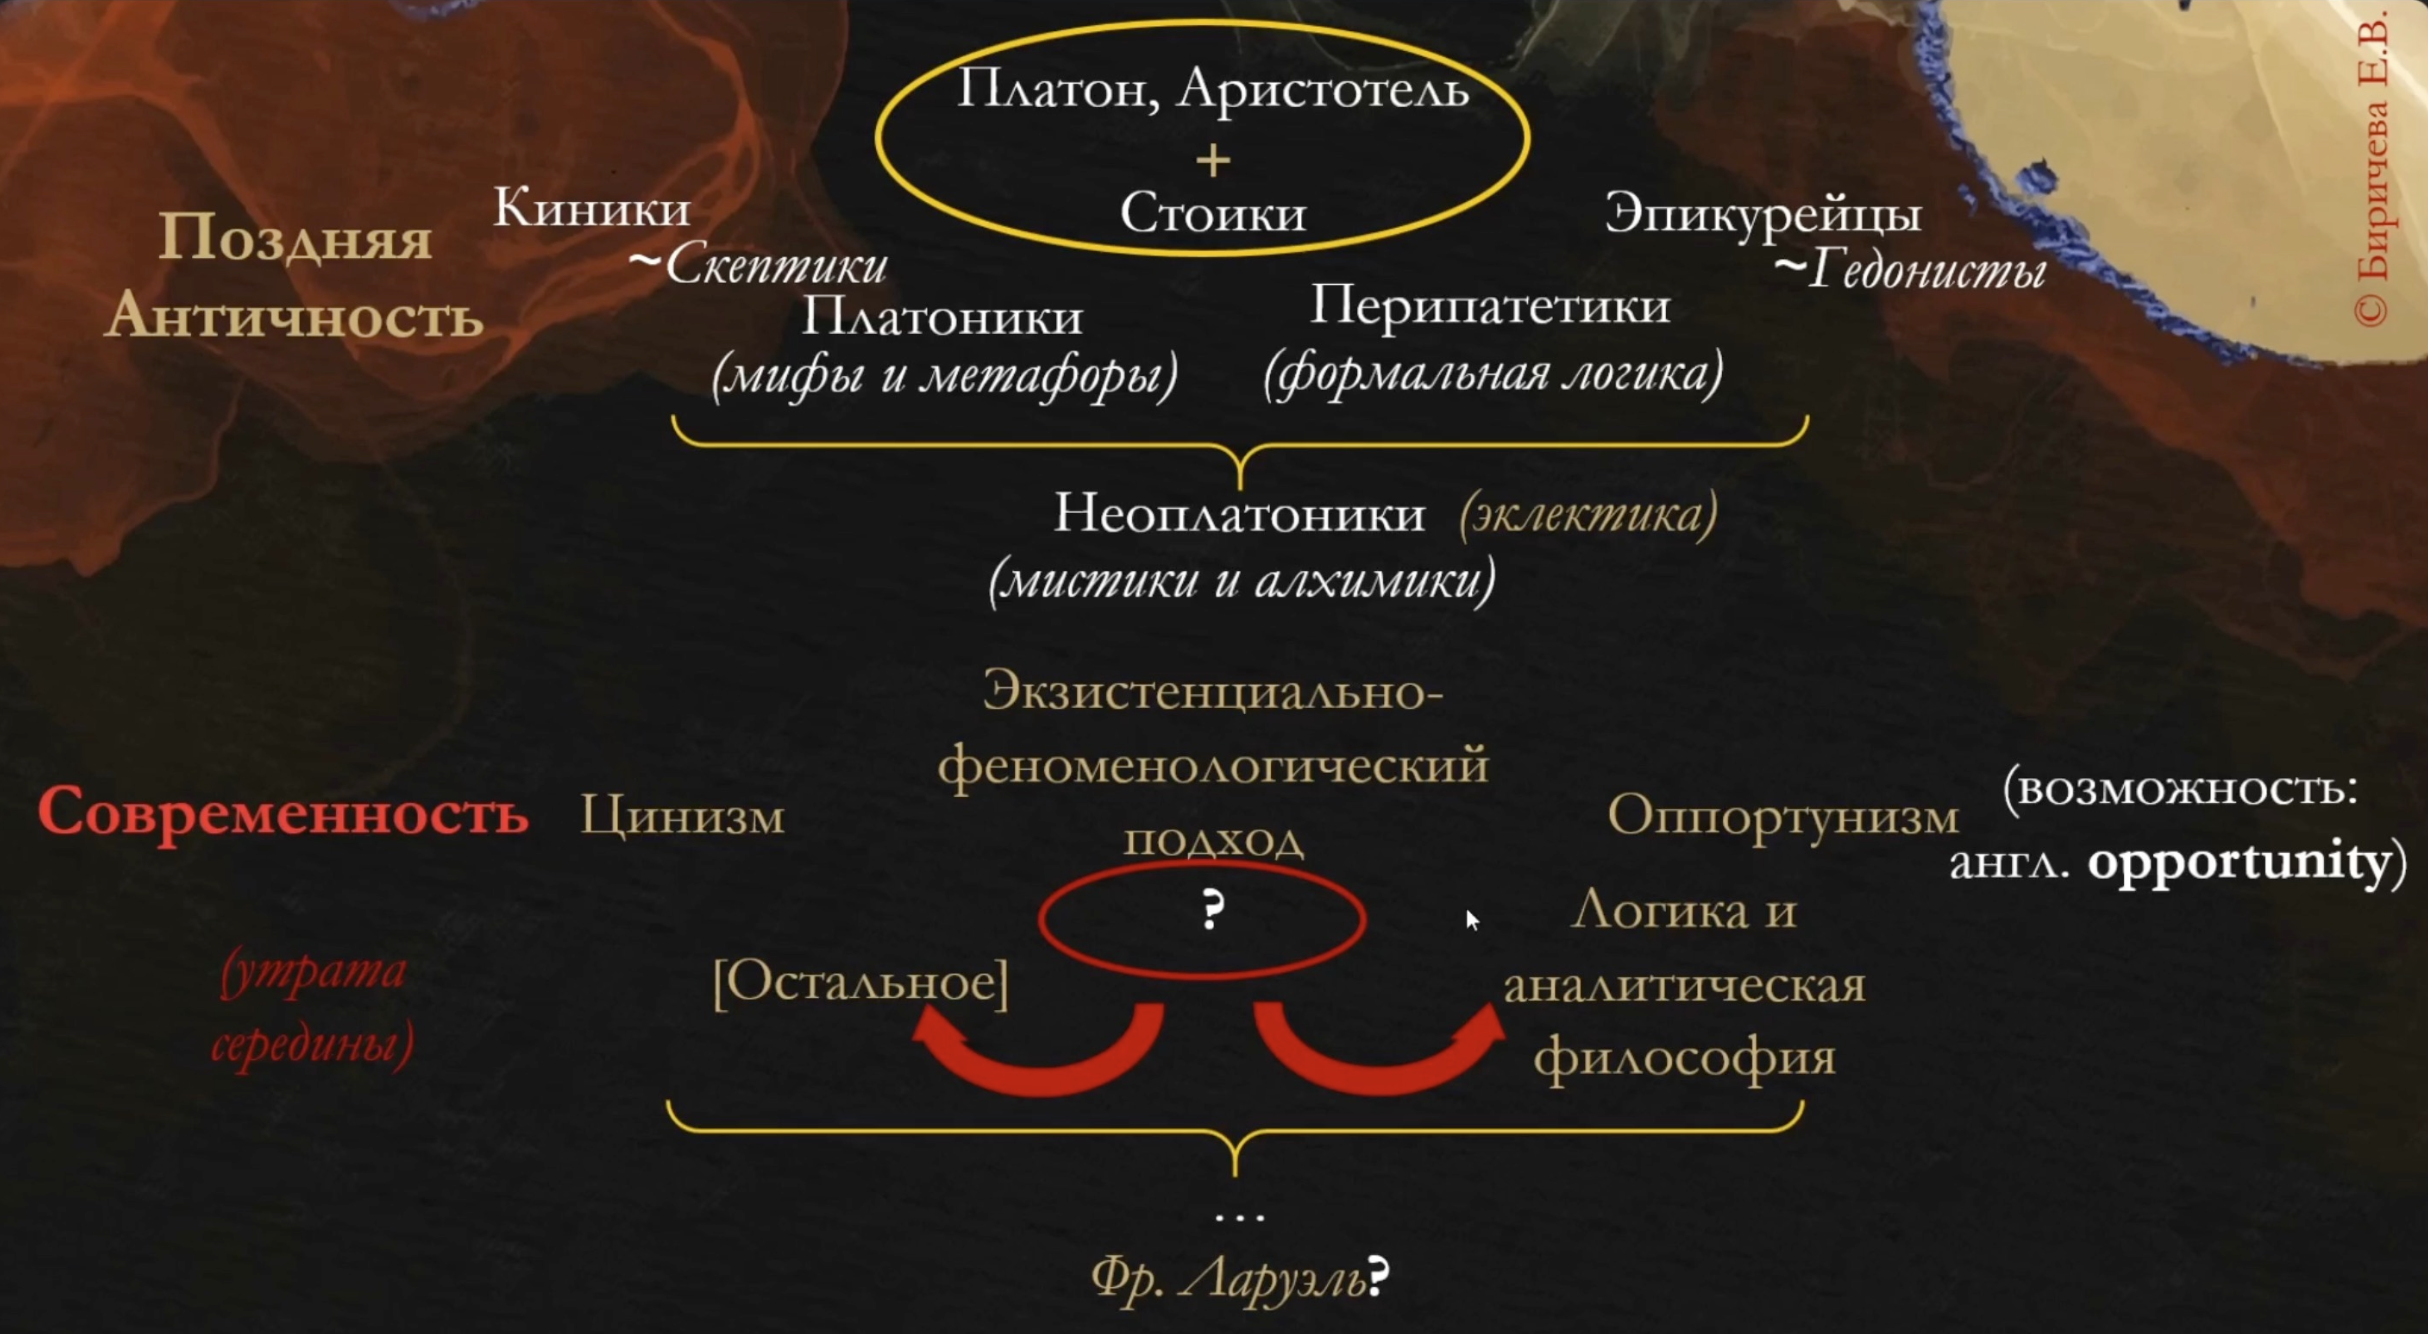
\includegraphics[width=0.8\linewidth]{pictures/archrev.png}
    \label{fig:archrev}
\end{figure}

Эпикурейцев часто упрощенно сводят к поиску удовольствий, а в эллинизме их философия стала символом индивидуализма. Киники же высмеивали саму культуру. Сегодня, как отмечал Бибихин, мы тоже переживаем возрождение Античности, но в отличие от нее теряем центр. Пауль Тиллих замечал, что стоицизм был единственным реальным соперником раннего христианства, а в современной культуре этой <<золотой середины>> почти нет. Неостоицизм~---~лишь бледная тень античных стойков, подогнанная под психологию и коучинг. Экзистенциально-феноменологический подход считают устаревшим, но нам нужно новое ядро~---~не эклектичное, а по-настоящему свое.

\subsection{Эпикурейцы, киники и стоики о метафизике, физике и этике}

% Теперь пробежимся по трем базовым направлениям, которые получили широкое распространение в период эллинизма и сохранили свое значение в ранней римской империи. Нельзя сказать, что какой-то из них лучше, какой-то хуже. Мы увидим сейчас, что у каждого своя правда. Каждое направление что-то схватывает в реальности, хотя часть может игнорироваться и замалчиваться, поэтому ни один подход не абсолютен. И то, что я лично люблю стоиков, не должно вас забивать с толку собственного решения о том, кто ближе именно вам. 

\subsubsection{Киники}

% Много рассказать не удастся, потому что в первоисточниках их не
% прочесть. Безусловно, представители киников писали свои философские
% трактаты, но поскольку их базовая идея постановка под вопрос всей культуры,
% отрицание и пренебрежение к сложившимся традициям и социальным ориентирам на них были гонения. 

% Это крайние маргиналы, смутьяны и оппозиционеры, которые
% критиковали любую власть. Поэтому никого из власть имущих не устраивали. Их
% сочинения изымались и сжигались. Кое-какие работы, например, основателя данного направления Антисфена дошли до нас, но это комментарии и интерпретации мифов о Прометее, Эрфее и Геракле, имеющие скорее филологическую направленность и не отражающие основ философского учения. 

Первичные источники киников почти не сохранились, так как их идеи, ставившие под вопрос культуру, традиции и власть, вызывали гонения. Их труды изымались и сжигались. До нас дошли лишь отдельные работы, например, комментарии Антисфена к мифам о Прометее, но они носят филологический характер и не раскрывают философской сути учения.


% Антисфен был рожден от рабыни, хотя отец всего был гражданином, но в древних Афинах незаконнорожденные не могли принимать участие в политической жизни. Учился он у Сократа, потому что тот не брал денег с учеников, а Антисфен по причинам своего происхождения был беден. Взял от Сократа он преимущественно идеи критики, постановки под вопрос текущих устоев. Из-за своего происхождения и желания равенства со свободными гражданами Антисфен открыто презирал сложившиеся культурные нормы и призывал других к переустройству общества. Поскольку он не имел средств для создания собственной школы, он начал с единомышленниками собираться в гимназии, там, где все желающие могли заниматься физкультурой, гимнастическими упражнениями на киносарге. Посмотрите на карте древних Афин, где располагались школы Платона, Аристотеля и Антисфена, а также где собирались стоики в крытой колонаде галереи или портики прямо около главной городской площади Агоры. Стоа~---~это название данного архитектурного строения. Ну, а киносарг~---~название холма в Афинах, на котором находился гимназий. В переводе оно означает <<зоркий пёс>> или <<белая собака>>. 

\paragraph{Антисфен} Родился от рабыни, хотя его отец был гражданином, но в древних Афинах незаконнорожденные не имели права участвовать в политической жизни. Он учился у Сократа, поскольку тот не брал денег с учеников, а сам Антисфен был беден. От Сократа он перенял прежде всего критический подход и привычку ставить под вопрос устоявшиеся порядки.

Желая равенства со свободными гражданами, Антисфен открыто презирал культурные нормы и призывал к переустройству общества. Не имея средств на создание собственной школы, он начал собираться с единомышленниками в гимнасии, доступной для всех желающих заниматься физическими упражнениями. 

Это происходило в Киносарге~---~гимнасии на окраине Афин. Название означает <<зоркая собака>> или <<белая собака>>.
% Так киников стали называть по месту их обучения, а они с радостью начали отождествлять себя с образом собаки, облаивающим всех вокруг, бродяжничающим животным. Если мы отрицаем культурный слой в человеке, что остается? Правильно, животное и вот природная естественность и её выживая сильнейшей стала идеалом киников. 
Киников стали называть так по месту их обучения, и они сами охотно приняли этот образ~---~собаки, которая лает на всех вокруг и ведёт бродяжнический образ жизни. Природная естественность и принцип <<выживает сильнейший>> стали для киников идеалом

% В своей жизни представители данной школы реально воплощали отказ от всех благ цивилизации, ходили практически голыми, не занимались никакими общественно полезными занятиями, жить старались практически под открытым небом и питались чем придётся. 
% Своими выходками они старались показать, что всё, что нормальный человек считает духовным и культурным, придуманное, пафосно, ничего не стоящее, ни на чём не держащиеся иллюзии. 

Киники на деле \textit{отвергали все блага цивилизации}: ходили почти нагими, не занимались общественно полезным трудом, жили под открытым небом и питались чем попало. Своим образом жизни они демонстрировали, что всё, что люди называют духовностью и культурой,~---~лишь надуманные, пустые иллюзии.

% Наиболее известен ученик антисфена Диоген Синопский, тот самый, который жил в огромном глиняном пифоне. Он прожил какое-то нереальное количество лет. Так ли это, не знаю, но в источниках стоят эти даты без пояснений, как он столько прожил с его образом жизни. 
% Диоген стал человеком-легендой ещё в древности. Приведу лишь штрихами к наброску его образа несколько фактов из его жизни. В случае вписано гораздо больше. Во время посещения Дельф пифия предрекла молодому Диогену переоценивать ценности, что он вначале понял буквально, начав заниматься фальшивомонетничеством. Обман раскрылся, и их с отцом изгнали из родного города. 
% Позже он осознал, что речь шла не о материальных, а о духовных ценностях. Перебравшись пытать счастье в Афинах, Диоген встретил Антисфена, который пытался выгнать его палкой из своей школы, просящего денег за обучение, которых у изгнаний естественно не было. Этот Диоген, снося его удары, ответил, бей, но ты не найдешь такой крепкой палки, чтобы прогнать меня, пока ты что-нибудь не скажешь. И учитель, узрев в этом идеал своей школы, все же оставил Диогена в гимназии. 
% После долгого пребывания в Афинах, Диоген начал странствовать по Греции. Во время одной из поездок его захватили пираты и продали в рабство коринфянину Ксениаду, который сделал его наставником своих детей. Новому хозяину Диоген заявил, что тот должен его слушаться, так же, как врача или кормчивый. Детей Ксениады он обучал литературе, истории, умению ездить
% верхом и владению оружием. Дети полюбили своего наставника и заступались за него
% перед родителями, когда тот выкидывал очередную эпатажную выходку. Когда в
% Каринфе находился Александр Македонский, к нему приходили многие политики и
% философы. Царь Македонии предполагал, что среди прочих его посетит Диоген.
% Однако философ спокойно проводил время в пригороде, нисколько не интересуясь
% присутствием в городе Александра. Тогда царь решил посетить Диогену сам. В это
% время философ угрелся на солнце, слегка приподнявшись при виде множества
% приближающихся людей, Диоген пристально посмотрел на Александра. Царь сказал,
% проси у меня чего хочешь. Но что Диоген ответил, отойди, не заслоняй мне солнце.
% Царь был настолько поражен гордостью и величием философа, который отнесся к нему с таким пренебрежением, что на обратном пути сказал, если бы я не был Александром, я хотел бы быть Диогеном. 

\paragraph{Диоген Синопский} Был самым известным киником, жил в огромном глиняном пифосе. Он стал легендой ещё при жизни.

Юному Диогену в Дельфах предсказали, что он должен <<переоценить ценности>>. Вначале он понял это буквально и занялся фальшивомонетничеством, за что его вместе с отцом изгнали из родного города. Позже осознал, что речь шла о духовных ценностях, и отправился в Афины, где встретил Антисфена. Тот пытался прогнать его палкой, но Диоген стойко выдержал удары, заявив: <<Ты не найдёшь такой крепкой палки, чтобы прогнать меня, пока не скажешь что-то стоящее>>. Антисфен признал его достоинство и принял в школу.

Во время пребывания Александра Македонского в Коринфе философ нисколько не интересовался его приездом. Тогда сам царь пришёл к нему и спросил, чего бы тот хотел. Диоген, загорая на солнце, ответил: <<Отойди, не заслоняй мне свет>>. Поражённый его независимостью, Александр сказал: <<Если бы я не был Александром, я хотел бы быть Диогеном>>.

Аскетизм Диогена не был отказом от всех благ и не предполагал самоистязания. Он отвергал лишь те потребности, удовлетворение которых требовало компромиссов и ограничения свободы. Этот принцип назывался \textbf{автаркией}~---~самодостаточностью, независимостью от внешних условий.

% Аскетизм Диогена не предполагал самоистязания и отказа от всех житейских благ. Он отрекся от тех потребностей, удовлетворение которых требовало компромисса, отказа от свободной жизни. Это называется авторкия, самодостаточность, предполагающая независимость от внешних условий. 

% Диоген мог посещать богатых людей и участвовать в их пирах, сохраняя
% свое оскорблявшее хозяина непристойное поведение. Когда философа привели в
% роскошное жилище и запретили плевать на пол, то он плюнул в лицо хозяину,
% заявив, что хуже места не увидел. Когда ученые-мужи разбирали апории Зенона,
% восхищаясь тем, как элеец показывает невозможность движения, Диоген встал и
% молча стал ходить взад-вперед, самим своим действием демонстрируя движение.
% Однажды Диоген днем зажег фонарь и пошел по улице. На вопросы, что он делает,
% следовал ответ <<ищу человека>>. Здесь прокомментирую отношение к парадоксам. В
% реальности нет человека вообще. Мы всегда либо мужчина, либо женщина. Так же,
% как в момент <<теперь>> никогда не зафиксировать целиком, что такое сутки, либо
% день, либо ночь. Рука или правая, или левая. Нет руки вообще. Так что выходкой с фонарем мыслитель продемонстрировал, что наших представлений человека вообще в действительности днем с огнем не найти. Это касается платоновских эйдосов.
% Вообще его бесило учение Платона. На шуточное определение в одном из платоновских диалогов, что человек есть животное на двух ногах лишенное перья, Диоген ощипал петуха, объявив, что это есть платоновский человек. Удивительно, но этого чудака одаривали своим вниманием по собственной воле лучшие гетеры Афин. Вообще все здесь взрослые детишки, поэтому будем смотреть на всю полную картины. контент 18+, ребят, и Диоген, и другие последователи школы киников, а их было немало, вплоть до окончания античной эпохи, и среди них были женщины, совершали не только эксцентричные поступки, но и публично бесстыдство и непристойности сексуального характера. Так в исторических источниках передают, например, что в ответ на разговоры о концепции платонической любви Диоген начинал публично онанировать. Срамота, конечно, и все подобное стойки, например, очень критиковали, хотя, скажем, разделяли идею внутренней независимости автаркии, но были сторонниками общественно адекватных проявлений.

% В политическую науку Диоген ввел понятие космополита или гражданина мира. Идея для античного мира была революционной, так как граждане Эллады ассоциировали себя с определенным полисом. Диоген отрицал понятие отечества и местных законов, утверждая, что есть только один закон природы, которому необходимо следовать.

Диоген ввел в политическую науку понятие <<космополита>> или гражданина мира. Эта идея была революционной для античного мира, поскольку граждане Греции традиционно ассоциировали себя с конкретным полисом. Диоген же отвергал понятие отечества и местных законов, утверждая, что существует только один закон~---~закон природы, которому следует подчиняться.

\subsubsection{Эпикурейцы}

\paragraph{Эпикур}

% Эпикур родился на острове Самос в Эгейском море. Его родители были уроженцами Афин. После прохождения военной службы Эпикур присоединился к своей семье, изгнанной после смерти Александра Македонского в Малую Азию. 
% получил разностороннее образование, учился риторики, а также философии у ученика Платона, пифагорейцев, затем у последователей Демокрита. 

Эпикур родился на острове Самос, его родители были из Афин. После службы в армии он присоединился к семье, изгнанной в Малую Азию после смерти Александра Македонского. Получил разностороннее образование, учился риторике, философии у ученика Платона, пифагорейцев и последователей Демокрита.

% В возрасте 32 лет Эпикур основал свою школу
% сначала на территории современной Турции, а затем в 306 году до нашей эры
% переехал в Эфиме, купил там сад и обосновался в нем со своими учениками. Поэтому эпикурейцев также называли философы сада. Над входом висело изречение гостя, теперь здесь будет хорошо, здесь удовольствие и высшее благо. Эпикур открыто
% позволял всем желающим, в том числе женщинам и рабам, вступать в свою школу. 

В 32 года Эпикур основал свою школу в Малой Азии, а в 306 году до н. э. переехал в Эфес, купил сад и обосновался там с учениками. Поэтому эпикурейцев называли философами сада. На входе висела надпись: <<Здесь будет хорошо, здесь удовольствие и высшее благо>>. Эпикур принимал всех желающих, включая женщин и рабов.

% Из более чем 300 произведений, которые, как предполагает, написал Эпикур,
% сохранились всего три письма Геродоту к Пифоклу и к Никею. Два спорника
% афоризмов и некоторые фрагменты, которые удалось восстановить из цитат других авторов.

% На глазах Эпикура происходил крах привычной социокультурной среды
% греков, и мыслитель чувствовал нарастающую тревожность и дезориентированность в
% умнострениях соотечественников, поэтому решил, что целью его философии будет
% помощь людям в достижении счастья и безмятежной жизни. Как же достичь в таком
% нестабильном плюралистичном мире удовлетворенности и спокойствия, как
% освободиться от страхов? Такая отрешенная безмятежность называется атораксией.

Эпикур стал свидетелем краха привычной социокультурной среды греков и почувствовал тревогу за умственное состояние соотечественников. Он решил, что целью его философии будет помощь людям достижения счастья и безмятежной жизни. В таком нестабильном мире удовлетворенность и спокойствие можно найти через освобождение от страхов. Такая отрешенная безмятежность называется \textit{атараксией}. 

По Эпикуру она предполагает отсутствие беспокойства, прежде всего о собственной смерти и других тревожащих вещах, таких как политический строй, устройство мира или выбор ценностных ориентиров. 

Эпикур считал, что лучшая жизнь~---~это самодостаточность в кругу друзей, комфортом и минимизацией телесных страданий, социальных конфликтов и морального перенапряжения.  Он утверждал, что нужно разумно подходить к удовольствиям: одни необходимы для удовлетворения базовых потребностей, а другие могут привести к проблемам, как болезни или зависть окружающих. 

Эпикур был первым, кто предложил не смущаться множественностью объяснений природных явлений, а не волноваться из-за этого, если наши объяснения помогают нам ориентироваться в мире.

% Она по Эпикуру предполагает отсутствие беспокойства, прежде всего о собственной
% смерти, а также о других тревожащих нас вещах, о том или на политическом строе,
% о том, как объяснять устройство мира, о выборе ценностного ориентира и так
% далее. Эпикур стал тем, кто впервые предложил не смущаться множественности
% возможных объяснений природных явлений и учел не волноваться из-за этого, лишь
% бы наши объяснения помогали ориентироваться в мире. 

% Что касается основного
% ценностного ориентира, Эпикур утверждал, что лучше всего проживать
% самодостаточную жизнь в окружении друзей, вкусно кушая и уменьшая свои телесные
% страдания и боли, не ввязываясь в социальные конфликты и морально не
% перенапрягаясь. Конечно, не следует стремиться ко всем подряд удовольствиям,
% надо рассудительно смотреть, ведь одни из них, как ученый мыслитель, необходимы
% для удовлетворения обязательных потребностей, а без других можно прожить. Да и
% некоторые услады могут привести к болезням или накликать беду в форме зависти
% других, тогда человек не сможет быть в безопасности или будет телесно страдать
% больше, чем удовольствие получил. В общем, в этом плане надо быть дальновидными.
% Эпикур уловил, что корень всех человеческих неврозов заключается в отношении к
% смерти, предполагающем, что смерть ужасна и болезненна. Это приводит к ненужному
% беспокойству, эгоистичному самозащитному поведению и лицемерию. Согласно
% Эпикуру, со смертью тела душа тоже перестает существовать, и поэтому смерти не
% следует бояться. Мы не можем изменить этот природный закон, поэтому нужно просто
% спокойно принять его и перестать бояться неизбежного, сосредоточившись вместо
% переживания страхов на простых доступных благах. Поскольку для Эпикура есть
% только эта жизнь в этом мире, поэтому и следует прожить ее максимально приятно,
% минимизируя беспокойство и телесную боль. 



% Эпикур также полагал, что корень человеческих неврозов кроется в страхе перед смертью. Он утверждал, что смерть~---~это конец существования души, и бояться ее не стоит. Нужно принять этот факт и сосредоточиться на простых радостях жизни, стремясь к счастью, избегая лишнего беспокойства и боли.

% Боги, даже если они есть, в каком-то
% высшем мире вряд ли станут участвовать в человеческих делах и влиять на судьбу.
% Зачем таким благим существам замечать вообще наше низменное бытие? однако
% согласно учению Эпикура вести себя этично необходимо не потому что боги накажут
% или наградят нас за наши поступки, но потому что аморальное поведение будет нас
% же самих обременять чувством вины или навлекать лишние неприятности, отягощая и
% омрачая нашу жизнь, в которой следует стремиться к позитивному покою и духовному
% наслаждению. Так что эпикурейцы в отличие от киников были полными конформистами
% в отношении внешних социокультурных условий и концентрировались напротив на
% достижении максимального личностного комфорта. 

Эпикур считал, что боги, если они и существуют, вряд ли вмешиваются в человеческие дела. Они слишком далеки от нашего земного существования, чтобы заботиться о нас. При этом этичное поведение нужно не потому, что боги нас накажут или вознаградят, а потому что аморальные поступки приведут к чувству вины и лишним неприятностям, мешая нам достичь спокойствия и наслаждения.

\paragraph{Тит Лукреций Кар}
% Наиболее стройно и
% последовательно философию эпикурезма излагает римский мыслитель Тит Лукреций
% Кар. Данные о его жизни достаточно скудны, но, например, из биографии
% исследователей известно, что он ввел исторические представления о каменном,
% бронзовом и железном веках не только в натур, философию и психологию внес
% научный вклад. Прежде всего Лукреция известен своим произведением о природе
% вещей, состоящим из шести глав и написанным полностью в стихах. Учение
% эпикурейцев о достижении безмятежности и душевного комфорта на самом деле
% базируется на их физике, которая, в общем-то, неотличима от метафизики. Следуя
% атомистическим представлениям Демокрита, эпикурейцы утверждают, что всё, в том
% числе души, состоят из атомов и пустоты. В природе происходит непрерывное
% движение мельчайших частиц, сталкивающихся друг с другом случайным образом и
% образующих то одни, то другие комбинации. То есть, во-первых, причинность
% абсолютно случайна, хотя мы наблюдаем в природе закономерности, которые
% объясняются разнообразием как самих атомов, так и практически бесконечными
% возможностями их многообразных комбинаций. Во-вторых, происходящие на уровне
% атомов процессы, в том числе в наших телах, дают нам непрерывные ощущения,
% сменяющие друг друга в зависимости от нашего взаимодействия с окружающей средой.

Философию эпикурейцев чётко изложил римский мыслитель Тит Лукреций Кар в произведении "О природе вещей". Он ввёл понятия каменного, бронзового и железного веков и внёс вклад в философию и психологию. 

Эпикурейцы, следуя атомизму Демокрита, утверждают, что всё состоит из атомов и пустоты. В природе происходит \textit{случайное} столкновение частиц, образующих различные комбинации. Это объясняет наблюдаемую закономерность. Процессы на атомном уровне создают наши \textit{ощущения}, изменяясь в зависимости от взаимодействия с окружающей средой.

% Наконец, объяснение всего через движение чтец материи позволяет обосновать
% представление эпокурейцев о смертности души и о том, что этой смерти не следует
% бояться. Если для нас нет ничего, кроме ощущений, и вся наша эмоциональная и
% разумная деятельность берется из процессов на микроуровне, происходящих в телах,
% то, как только тело разлагается, мы перестаем что-либо ощущать, поэтому сама
% смерть не болезненна и не является страданием. Следовательно, как в третьей
% книге своей поэмы подробно разбирает лукреция, если человек жил и наслаждался
% своей жизнью, соответственно, он постиг и наивысшее наслаждение познания природы
% вещей и понял, что смерть природный закон. Надо расстаться с жизнью, чтобы из
% наших атомов что-то другое переродилось и создалось. Если же человека при жизни
% постигли несчастье и он не смог с ними справиться, а в старости его одолевают
% болезни, то тем более какой смысл держаться за такую жизнь, которая не приносит
% удовольствия. 

Эпикурейцы объясняют смертность души через движение материи: всё, что мы \textit{чувствуем},~---~это результат процессов на микроуровне, происходящих в теле. Когда тело разлагается, мы перестаем \textit{ощущать} что-либо, а значит, смерть не является страданием.  

% И последний момент, который хотелось бы чисто примечанием
% отметить, это эпикурейцы на основании атомистического учения ещё и обосновывали
% возможную множественность миров. В других вселенных атомы ведь могли бы иначе
% складываться в комбинации. Также наша вселенная вполне вероятно, что возникла
% когда-то и в какой-то момент может разрушиться. 

Опираясь на атомизм эпикурейцы объясняли возможность \textit{множественности миров}, утверждая, что атомы могут комбинироваться по-разному в других вселенных. Также они считали, что наша вселенная могла возникнуть и, возможно, когда-нибудь разрушится.

% Думаю, подобные воззрения близки многим нашим современникам, и я не раз общалась с такими коллегами физиками, химиками, биологами, разделяющими оказывается эпикурейские идеи о природе материи, причинности вселенной, множестве возможных миров и о выводах из этого для собственной борьбы со страхом смерти. Почему бы и нет, если это продуктивно?

\subsubsection{Стоицизм}

Стоицизм зародился тоже ещё в начале эпохи эллинизма, однако наиболее глубокое и
последовательное учение создали в более поздний период римские стойки.

Для
ранней Римской империи характерны централизация и военный характер власти, в
связи с чем социальной элитой становятся воины, образ жизни и задачи, которым
должны были обрести концептуализацию в особых ценностно-этических учениях. 
На эту роль не годились позиции ни киников, ни эпикурейцев,
поскольку первые отрицали власть и культурные нормы вообще, а вторые предлагали
уединиться в небольшом кругу друзей, наслаждаясь простыми благами, познавая
природу и не участвовав в социально-политических делах. Если эти стратегии не
подходят в окружающей неясности вектора общественного развития и объективных
опасностей, человек обнаруживает, что в своем понимании действительности в своих
поступках и суждениях опереться вовсе не на что. 

Естественно, тогда искать опору
в себе. Принятие всего обоих полюсов противоположностей, вдвинутых прежде
всего в существо самого человека, означает не только позитивный ряд добра,
красоты, разумности жизни, но и включение в свой горизонт страшного, злого,
безобразного, в том числе и смерти, своей прежде всего. Вроде бы эпикурейцы
нашли способ избежать страха смерти, но если мы присмотримся внимательнее,
окажется, что их решение всего лишь очередная иллюзия, которую мы не можем на
опыте не доказать, не опровергнуть. 

% Можно утверждать, что всё является
% взаимодействием атомов, но как тогда объяснить свободу моей воли? Хорошо, пусть
% наша душа распадается со смертью тела, но где гарантия, что мы перестаём ощущать
% после смерти, пока абсолютно все клетки тела не разложились? Да и вообще,
% природа природой, а может быть, я просто не хочу умирать, может, я ещё хочу что-
% то успеть, да и откуда тогда у других людей представление о загробной жизни?
% Почему я должна соглашаться с тем, что главное в жизни удовольствие и
% минимизация боли? Я бы не стала за это умирать, значит, это не главная ценность?
% Кстати, это хорошая самопроверка задуматься над тем, ради чего вы бы отдали
% жизнь. Это и будет ваш базовый ценностный ориентир. Легко ли тогда принять
% собственную смертность, когда мы видим, что не знаем, как всё на самом деле?
% Легко ли согласиться с этим природным, безусловным и не от нас зависящим
% законом? Нет. Но это нужный шаг, только такой, который никакие объяснения не
% подсовывает туда, где их не может быть, к тому, о чём у нас не может быть опыта.
Как принять смерть? На
такое мужество способны только отчаянные единицы, и по сути, это путь воина.
Так, стоицизм в Римской империи стал основанием мировоззрения прежде всего
немногочисленной воинской элиты, полководцев и императоров. 
% Как в другой
% культуре говорит о том же самом японский самурай Ямамото Цунутону, один из
% создателей бушидо-военного канона самурайского сословия, в действительности
% соответствовать этому пути способен лишь один из тысячи, ведь каждый норовит
% избежать работы, которая требует приложения усилий. Поэтому же 
Римский стоик,
выдающийся политический деятель своего времени Луциан Исенека, уверен, что, ища
подлинность жизни, нельзя следовать за общественным мнением большинства. 
% С
% такого предельного мужества самостоятельно смотреть реальности в лицо и принятие
% ее во всей полноте и парадоксальности берут свое начало стоицизм и бушидо. Общая
% для этих учений основополагающая метафора <<жить так, словно уже умер>> имеет
% огромную освобождающую силу. Несмотря на труд, усилия, применение этой формулы
% по отношению к себе она дарует независимость от всего, как внешнего, так и
% внутреннего. Живущий словно уже умер, человек не нуждается ни в чем, не спешит и
% не суетится, не зависит от еды и интересного комфорта, не привязывается даже к
% самым дорогим во всех смыслах вещах, людям, к местам, воспоминаниям, планам и
% так далее. Но такая свобода не произвол, не отрешенность. Этимологически свобода
% одно со своим собственным, не в более узком смысле моего частной собственности,
% а в широком, чьям и собственность, чему мы принадлежим. Вспоминаем самое само
% Платона. Оно через каждого течет уникальным способом и соответствием своему
% способу быть для конечного времени и пространства существа как раз означает
% максимально возможную полноту, интенсивное исполнение, самореализацию.
% Сложнейший путь, узнай себя, гнозис и автон, приводит к пониманию, что я не мои
% вещи, тело, переживания или представления, а уникальный способ быть.
% Следовательно, принципиально свободны от всего иного и способны на полноту в
% своем месте, независимо от наличия или отсутствия богатства, добра, славы и так
% далее. Попытки достичь полноту экстенсивно за счет чужого, завладения,
% уничтожения или бытия не своим способом, обречены на провал, поскольку уводят от
% единственного подлинного источника полноты, своего собственного. Вот об этой
% свободе, внутреннем, единственном надежном основании и учат стойки, а трудность
% золотой середине, которую нужно устанавливать, вопреки растаскивающим стороны
% противоположностям, независимо от внешних обстоятельств и внутренних
% переживаний. 
% Как пишет переживший в своей карьере взлеты и падения, в своей
% жизни болезни и изгнания, равно как богатство и почет, римский сенатор Сенека в
% письме к выдающемуся оратору, консулу Галеону: неважно,
% обеспечат ли ему перины и мягкие подушки, или же придется склонять уставшую
% голову на солому, будет ли его почитать царем или придется прислуживать кому-то
% на чужбине; ни богатство, ни благо, ни комфорт, ни почет не сделают его более
% счастливым, чем он сам себя может сделать, равно как и отсутствие этого всего не
% сделают его ни униженным, не оскорбленным, ни менее счастливым. Однако,
% безусловно, умный человек не станет отказывать себе в комфорте или невежливо
% относиться к тем, кто его уважает и почитает, поэтому нет смысла специально себя
% истязать и бежать от общества. Если будет выбор, то стоик возьмет лучшее, хотя
% он может обойтись и без всех благ, и даже в изгнании и бедах не потерять честь и
% достоинство. 

В отличие от эпикурейцев, стойки не относят богатство,
удовольствие, комфорт к высшим ценностям и благам, ради которых только стоит
жить. Хорошо, если они выпали на долю, но и без этого надо уметь обходиться,
если не выпало. 

В отличие же от киников, стойки не считают, что, с другой
стороны, для достижения внутренней свободы следует обязательно презреть
материальные, социальные и культурные ценности. Все это внешнее, как благо, так
и лишение этих благ. 
Настоящая свобода поэтому не может зависеть ни от статуса человека, ни от уровня достатка, ни от приятностей или их отсутствия. 

\paragraph{Марк Аврелий Антонин}

Император Марк Аврелий Антонин иногда делал небольшие заметки, которые в течение его жизни составили небольшой философский дневник, переиздаваемый до сих пор под названием <<Размышления>>. 

% Я не могу это читать без слез уважения к человеку, который был
% верховным правителем, не зависящим от наличия у него огромных богатств, военной славы, который обладал властью над несметным количеством людей, но при этом
% старался каждому помочь, о каждом заботиться и, как он сам себе напоминает в
% своих заметках, каждому воздать справедливо, по достоинству каждого. 

Император записывает для себя: <<Как ты относился до сих пор к богам, родителям, братьям, жене, детям, учителям, дядькам, друзьям, домашним, грабам? Ко всем ли у тебя до сих пор получается не совершить ничего беззаконно и не сказать? Вспомни и то, что ты уже прошел, и на что тебя уже хватило, и что теперь полное у тебя знание жизни, и что это последнее твое служение, и сколько прекрасного ты видел, и сколько раз пронебрег наслаждениями или болью, сколько славы не взял, к скольким недобрым был добр>>. 

Удивительный правитель Марк Аврелий понимал, что всем мил не
будешь, но ведь поступать стоит не ради мнения других, но на пользу своему
народу достойно выполняя свой долг, соответствует должности, которую ему
доверили. В таких случаях приходится своим желаниям и склонностям наступать на
горло, поскольку в дела императора входит судить и казнить преступников, даже
если тебе по-человечески их жалко, воевать с непокорными, даже когда не хочешь
проливать кровь, указывать другим и принимать решения, даже если сам не изучил
вопрос до конца, или когда хочется, чтобы все эти нескончаемые дела закончились,
и люди дали побыть наедине с собой, дали просто отдохнуть. 

Марк Аврелий пишет,
<<Гордыню оттеснить можно, одолевать наслаждение и боль можно, быть выше славы их
можно, на бесчувственных и неблагодарных не гневаться, а еще заботиться о них
можно>>. 

Пол жизни император мучился от язвы желудка и кровохаркания, тогда эту
болезнь не умели лечить, и это действительно в телесном плане очень мучительно.
Сначала Марк Аврели принимал сильнодействующее обезболивающее, но потом понял,
что это наркотик, и не желая погубить ясный ум, выбрал испытывание боли и мук в
противоположность утрате самоконтроля. 

% Он пишет в своих заметках, что все
% подобное происходит по природе, но от нашей воли зависит, мужественно ли мы
% принимаем беды, продолжаем ли вопреки им заниматься необходимым своим делом,
% остается ли свободной наша душа. Так вот, пусть не идет извне признание, и все у
% тебя хорошо, и если даже это тело твое режут и жгут, если оно гниется, гниет,
% пусть та доля, которая ведает признанием этого, будет покойна, то есть пусть так
% рассудит, что это не добро, не беда, раз может так случиться и с хорошим
% человеком, и с дурным, ты душа на себе труп таскающий. И вот еще с другого места
% его книги. Быть похожим на утес, о который непрестанно бьется волна, он стоит, и
% разгоряченная влага затихает вокруг него. Несчастный я, такое со мной случилось,
% нет, счастлив я, что со мной это случилось, а я по-прежнему беспечален,
% настоящий в него изъявлен перед будущим неробею, случиться-то с каждым могло
% такое, но беспечальным остаться сумел бы не всякий. Так запомни, во всем, что
% наводит на тебя печаль, надо опираться на такое положение, не это несчастье, а
% мужественно переносить это счастье. Свобода способа бытия, решающаяся на весь
% размах между полюсами и противоположностями, требует непрестанной борьбы с
% собой, как со страхом небытия, так и со своими непродуктивными желаниями,
% надеждами, иллюзиями, уводящими от полмуты. Главные враги тогда не вовне, а
% внутри, не научившись побеждать такие свои пороки, как вожделение, гнев,
% зависть, жажду наживы, гордыню, действия из личных интересов и выгод, лень и так
% далее. Вряд ли человек сможет противостоять превратностям судьбы или другим
% людям. Эти негативные черты можно также переселить упором на противоположное,
% взращивая в себе, постоянно практикуя добродетели, главная из которых
% рассудительность, искренность, мужество, верность в себе, внимательность, ко
% всему, в том числе, к деталям, мелочам, сострадание, самообладание, умение
% терпеть страдания, целеустремленность. Однако полнота предполагает не смесь
% противоположностей, но удерживающую баланс между ними золотую середину. Поэтому
% важно не стараться всегда быть праведным, но думать только о пути, для чего
% нужно научиться умело отходить от нормы и не имея предпочтений к определенным
% чертам, стилям, характеристикам, поступать сообразно текущему моменту. 

Полнота
бытия означает не только предельный охват возможного, но и, самое главное,
присутствие происходящего в
действительности. Реальное, подлинное, настоящее может быть достигнуто в
концентрации на том, что здесь и теперь. Нет ничего за пределами текущего
мгновения. Прошлого уже нет, можно только извлечь из него опыт, но держаться за
него и копаться в нем бессмысленно. Будущего еще нет. Сколько бы мы ни строили
планов и ни предполагали, практически все во власти непредсказуемой судьбы. 

И поскольку вся жизнь человека есть последовательность мгновений, как пишет
непрестанно преодолевавший страх смерти Марка Аврелий, каждый жив только в
настоящем мгновении. Если мы полностью собрали себя в настоящем, нам нечего
терять и не о чем беспокоиться, если пребываем в готовности чувствовать, когда и
что пора, и поступать в сообразной реальности. 

Пребывание здесь и теперь
связывается за внимание у Марка Аврелия об этом чуть ли не на каждой странице. В
присутствии, при сути происходящего человек превращается в чуткое видение того,
что есть. Такое видение противоположно веданию, как состилающему настоящему
рассчитывающему представлению, плану, набрасыванию ярлыков, попытке уместить
реальность в схему. Несмотря на то, что постоянное обучение и
самосовершенствование важны, как воздух, бывают случаи, когда многие знания
оказываются препятствием. Здесь наши авторы не противоречат себе. Для всего есть
своя пора. Для учения, чтобы приобрести знания и натренировать способности, и
для участия в событиях, в рамках которых губительно рассуждать, как быть, когда
они уже происходят и требуют единства с собой. Поэтому учат они не столько
конкретным техникам, сколько внимательности к настоящему, отсекая все лишнее,
рассеивающее, глубоко входить в каждое действие, сообразовываться с реальным,
без плана, без представления. На фоне решительного принятия временности своего
бытия внимательность к настоящему вплоть до мельчайших деталей открывает и
пронзительную полноту прекрасного, которую можно увидеть во всем. Даже, как
пишет Марк Аврелий, в неровной корочке хлеба, звериный морг гнущихся осенних
колосьях или морщинистой кожи пожилого человека. 

\paragraph{Луций Анней Сенека} начинает свою физику с вечных философских вопросов и с упоения той красотой, которая заключена не
только в видимом, но и зашифрованном в законах природы. Так, видение красоты во всем, стремление к высшему познанию вселенского порядка и принятие естественного течения бытия определили идеалы жизни и поступков согласно с природой, ее законами и ритмами. 

Но стоики, в отличие от киников, в этом плане не
предполагали сведения всего человеческого в нас к животному. Природа составляет
огромную, не нами созданную, не нами управляемую часть реальности, которую
необходимо принять и которой нужно соответствовать. Это значит, в том числе,
принять особую природу человека, который, в отличие от животных, этическое,
способное рационально мыслить открытое и свободное существо. Поэтому следование
собственной природе означает прежде всего мужественно-рассудительное участие в
общественной, политической, культурной жизни. Так, неопределенности социальных
отношений и непредсказуемости объективных случайностей, стоицизм
противопоставляет свободу своего собственного исполнения в любом содержании
занятий, концентрацию, здесь и сейчас, целиком присутствия в том, на чем в
данный момент сосредоточен. Мы не можем изменить судьбу, но можем изменить
отношение к ней. На самом деле, реальность нейтральна, знамения имеют место лишь в глазах смотрящего. Даже, казалось бы, отрицательное лишение трудности можно увидеть как для чего-то нужное и полезное, как вызов для преодоления или как опыт для дальнейшего самосовершенствования. Наши авторы советуют буквально радоваться трудностям, поскольку без препятствий нет развития. Бедствия~---~самый удобный случай для проявления доблести, напоминает нам Сенека.

\subsection{Александрийский Мусейон: математика Евклида, механика Архимеда, неоплатонизм}

Созданный одним из диадохов Птолемеем I, в III веке до н.э. после
завоеваний Александра Великого, Александрийский Мусейон непрерывно функционировал в качестве уникальнейшего культурного и научного центра в течение почти 800 лет.

Его сохранили и продолжили поддерживать римские завоеватели уже в нашей эре, но закрыли только после окончательной христианизации в начале V столетия в связи с идеей борьбы с язычеством. А все работавшие в Александрии ученые были греко-римского или египетского происхождения и в основном следовали мифологическим представлениям своих народов. 

Идеологами создания данного комплекса и первыми служившими там исследователями были перипатетики~---~ученики Аристотеля.
Сам музей известен прежде всего обширной библиотекой, воплощавшей желание Птолемея создать у себя хранилище всех знаний, чтобы привлекать и воспитывать в своем государстве лучшие умы. В библиотеке продолжали столетиями накапливать книги выдающихся ученых и философов, как работавших в Александрии, так и известных авторов из других, в том числе арабских и азиатских стран. 

Кроме, так сказать, беспрецедентного по своему замыслу международного информационного центра, на территории были разбиты ботанические и зоологические сады, создана техническая выставка автоматических устройств, открыта медицинская школа. Вплоть до властвования последней царицы эллионистического Египта, Клеопатры из рода Птолемеев, продолжалось также накопление коллекций художественных произведений и иноземных диковин. 

В ходе гражданских войн и внешних завоеваний несколько раз происходили пожары и разрушения, в результате которых части собраний книг и предметов искусства были утеряны. Однако, интеллектуалы спасали те произведения, которые могли, а властители старались восполнить коллекции и восстанавливали несколько раз этот уникальный культурный комплекс. 

В Александрии развивались математика и механика, филология и астрономия, география и история, минералогия и медицина. Именно здесь зародилась алхимия и системные теоретические основания металлургии. 
Возникла школа неоплатонизма. Этот мощный научно-образовательный центр породил на множество самых известных ученых и философов поздней античности, среди которых было также немало женщин, наряду с мужчинами, преподававших и издававших научные труды. 
Например, Мария Пророчица, первая женщина-алхимик, основательница алхимической школы, изобретательница ряда химических аппаратов и процессов, используемых по сей день. 
Гепатия Александрийская, женщина-математик, астроном, механик, философ и глава неоплатонической школы. Астрономическую систему, созданную во втором столетии Клавдием Птолемеем с неподвижной землей в центре космоса, примут как основополагающую почти на полторы тысячи лет и пересмотрят только в 16 веке благодаря Николаю Копернику и Галилеу Галилею.  
Альтернативы геометрии Евклида, разработанные в 3 веке до н.э., предложат только в 19 столетии. 

Важнейшими чертами Александрийской науки были, во-первых, энциклопедичность, собрание знаний обо всех сторонах действительности и попытки представить их на единых более или менее непротиворечивых основаниях. 
Второе, что бросается в глаза, это мощная практическая направленность исследований. В отличие от во многом умозрительного познания классической Греции, Александрийский научный центр задумывался с неплохой эмпирической базой, интегрировавшей также практические наработки восточных культур и нацеливающейся в том числе на полезные изобретения. Это был мудрый политический ход Птолемея. 

Таким образом, непревозойденная греческая теория ассимилировалась на почве практически ориентированного знания восточных культур, а правители получали не просто информационный библиотечный центр, которых в древнем мире было немало, в том числе у египтян, персов, ассирийцев, но самое главное базу научных открытий и технических изобретений. Впоследствии римская наука будет перенимать эти черты. 

Не в ущерб детально проработанной теоретической составляющей активно развиваются и применяются такие практические решения, как водопровод, акведук, водяная мельница, абак, прототип калькулятора, гиппокаус, утопительная система, сооружаемая под полом, механическая пила, специальная оптика с использованием зеркал для ночного освещения и маяков и множество других полезных изобретений.

Наконец, к особенностям Александрийского мусея относится и то, что это был фактически полноценный в современном смысле исследовательский институт. Он находился на попечении текущей власти, как эллинистической, так и затем римской. И трудящиеся там ученые, в том числе приезжающие на обучение иностранцы, получали жалования и отдельно премии за изобретение или полезные практические решения. Были учреждены литературные и художественные премии и награды для творивших там деятелей искусства. Также до начала третьего века члены мусея освобождались от налогов и, вероятно, от общественных повинностей. 

\subsubsection{Евклид}
В III веке до н.э. Евклид впервые предпринял попытку систематизировать все математические учения, наработанные античной мыслью за предшествующие несколько столетий, \textit{сводя их к единым основаниям}.
% Хотя и до него исследователи составляли книги, задержавшие обширные сведения о различных областях математики,
% Евклид занялся именно сведением всех учений к единым основаниям. 
Он знаменит сочинением <<Начала>> из 13 книг, в котором последовательно излагаются основы геометрии и теоретической арифметики, а также закладываются основы геометрической алгебры. 

% Этот труд более чем на два
% тысячелетия стал базовым учебником по геометрии. Математическое учение во многом восходящее к пифогорейцам. 
% На самом деле и в современной школе преподается, но все фактически обучались евклидовой геометрии с 5-6 по 10-11 класса. 
% Сегодня о неевклидовых геометриях иногда рассказывают только в 11 классе. В связи с этим мы не будем сейчас детально перечислять, что именно представляет собой основу геометрии и как эта дисциплина соотносится с арифметическими вычислениями.
% Единственное, что мы отметим, это философский принцип, в соответствии с которым Евклид систематизировал известные ему математические учения. 

<<Начала>> Евклида представляют собой образец системности и последовательности мышления, поскольку организованы логически путем выведения из базовых определений и положений важнейших следствий. 

Евклид несомненно опирался на философию Платона и Аристотеля в своем методе организации математического знания. Геометрические чертежи, на которых при проведении вспомогательных линий неявная истина становится очевидной, служит иллюстрацией для платоновской концепции \textit{припоминания}. 

Предложения геометрии потому и называют теоремами, что для постижения их истины требуется воспринимать чертеж не простым чувственным зрением, но очами разума, теоретически. Всякий же чертеж к теореме представляет
собой идею. 

Мы видим перед собой эту конкретную фигуру, а ведем рассуждение и делаем заключение сразу для всех фигур одного с ней вида. Также и без опоры на классическую логику Аристотеля и его аналитики, столь последовательное и логически верное рассуждение в рамках доказательства теорем не было бы возможно.

\subsubsection{Архимед}
Знаменитый древнегреческий математик, физик и инженер из Сиракуз на Сицилии.

Архимед, обучавшийся также в Александрии, во многом обязан систематизации
математики, осуществленной Евклидом. Труды Архимеда относились почти ко всем
областям математики того времени. В частности, работы по алгебраическому представлению объемных сечений, вычислению площадей и объемов сложных фигур способствовали развитию в дальнейшем математического анализа. 

Архимед прославился также изобретением различных механических устройств и конструкций, описав действие рычага, винта, поднимающего в воду, систем блоков для выигрыша в силе при поднятии грузов. В порту Сиракуз благодаря Архимеду работало множество блочно-рычажных механизмов, а город успешно оборонялся во время осады римлян созданными Архимедом метательными машинами. 

С жизнью Архимеда связано несколько легенд:
Широкую известность получил рассказ о том, как он сумел определить, сделана ли корона царя Гиерона полностью из золота, выданного царем для этого заказа, или нанятый ювелир сжульничал, подмешав в расплав серебро. Размышляя над поставленной задачей, Архимед пришел в баню и, погружаясь в ванну, обратил внимание на поведение уровня воды. В этот момент его осенила идея о соотношении вытесняемого объема и веса, которая легла в основу гидростатики. С криком <<эврика!>> Архимед выскочил из ванны и побежал проверять свою гипотезу. Сравнив объемы воды, вытесненные короной и слитком золота равного с ней веса, ученый доказал обман ювелира. 

Согласно другой легенде, благодаря открытию теории рычага и созданию полиспаста, Архимед смог в одиночку сдвинуть с места огромный корабль при перевозке его по суше на катках. Ошеломленным соотечественникам ученый сказал, что будь у него точка опоры, он бы перевернул Землю. 

Во время штурма Сиракуз римлянами устройства привели к поражению целой армии, которая атаковала город с моря и суши. Римляне, надеявшиеся быстро захватить город, были вынуждены отказаться от первоначального плана и перешли к осаде. Через два года город захватили, и то благодаря изменнику. Во время штурма Архимед, захваченный решением своих математических задач и не обративший внимания на ворвавшихся воинов, был убит на месте. 

Огромное наследие научных работ Архимеда по сей день активно изучается и систематизируется. Историки до сих пор в XX и XXI веках находят ранее неопубликованные труды великого математика и механика и удивляются
глубине и ширине его мысли. 

\subsubsection{Неоплатонизм}

Это новая жизнь платоновского учения, которую развили во II-III веках н.э.
александрийские исследователи. Они интегрировали теоретические положения
философии Платона с магически-мистической, алхимической и астрономической
практиками, а также синтезировали наработанные предшественниками знания 
аристотелевским методом. 

Основные положения неоплатонизма представлены в сочинениях Плотина. Работу учителя после его смерти собрал и систематизировал финикийский мыслитель Порфирий. Он организовал труды Плотина в шесть томов по девять трактатов~---~Эннеады.

% Плотин создал
% продуманную и самосогласованную систему представлений просто обо всём. 
% Иногда я
% перечитываю трактаты из этих его сборников и каждый раз не перестаю поражаться,
% как точно и логично у него всё сказано, как тщательно воедино собрано лучшее из
% Платона, Аристотеля и стойков, но при этом сказано новое своё. 

Согласно неоплатоникам, мир не является результатом специального замысла божеств или единого бога Демиурга, но появился в результате необходимости в средстве эманации, что значит нисхождений Единого, поскольку в основании всего мироздания Единое, которое обладает свойствами целостности, полноты и всеобъемлемости. Оно настолько богато своей полнотой, что переполняясь бытием и как бы желая бесконечно делиться собой, взрывается, выливается в огромный космос, гармоничный и мудро организованный. 

Единое эманирует в Ум, который у ранних мыслителей Нус и Логос, такой вселенский разум, или лучше сказать единая мысль обо всем, которая управляет Вселенной. 

Плотин убедительно доказывает, что само Единое непостижимо, и мы имеем дело только уже с дальнейшими как бы ступенями его выражений в форме Ума, порядка мирового целого и затем в виде Души Мира. 

Все существа являются как бы складками, постоянно движущиеся, бесконечно многообразные, чувствующие, на разные лады самовыражающиеся единой ткани Мировой Души, которая в каждом пытается найти удачную комбинацию. 

Так, ни одно существо полностью не умирает. При рождении просто перекомбинируются части этой единой Души Мира, пробуется новая вариация. Материя мыслится в такой системе в качестве самого низшего невоодушевленного начала, причем не существующего в действительности, но только в возможности. 

% Кто хочет поломать себе голову над парадоксом реального и потенциального несуществующей материи и существующих вещей, почитайте вот этот
% маленький трактатик под ссылки. Потом подобное тотчайшее рассуждение о том, что материя в пределе ничто можно найти только у средневекового Иоанна Дунса Скотта.

Что же касается человека в такой продуманной сложной системе вещей, он специфичен по сравнению с животными тем, что оказывается способен приобщиться к Уму и понимать фундаментальные законы и первопричины мироздания.

Однако часть нашей души отягчена животным началом, увязая в материи и для того, чтобы обрести настоящее человеческое счастье, надо возвысить душу при жизни.

Достигать возвышение своей человеческой души следует в единении со всей душой мира, затем в приобщении к разумению космического первопорядка ума и наконец в воззрении того истока единого, который непостижим, но о котором можно догадаться. 

Неоплатоники предлагают через практики самоочищения, аскезы и медитации очищать свою душу таким образом и возвышать ее. То есть на пути к счастью следует максимально отрешиться от всего материального, земного и устремить свой внутренний взор благодаря прилежно последовательно осуществляемому познанию к самым фундаментальным основам. 
Тогда и высшим блаженством становится само мышление, а главное добродетель, чистое видение всего, как оно есть, глазами разума. Неоплатоники поэтому отрешаются от социально-политической жизни, сосредотачиваясь на исследованиях и предпочитая познание основ мирской жизни. Такая выстраивается иерархия ценностей.

% Безусловно, хороши и нужны, гражданские, как их называют паутин добродетели,
% вроде мужества, щедрости, справедливости, но вообще-то это все необязательно.
% Главное добродетель интеллектуальная.
